\documentclass[12pt,a4paper]{report}

%==========================================
% Packages
%==========================================

\usepackage{graphicx}
\usepackage{float}
\usepackage{amsmath}
\usepackage{amssymb}
\usepackage{booktabs}
\usepackage{multirow}
\usepackage{array}
\usepackage{longtable}
\usepackage{tabularx}
\usepackage{caption}
\usepackage{subcaption}
\usepackage{enumitem}
\usepackage{hyperref}
\usepackage{geometry}
\usepackage{setspace}
\usepackage{fancyhdr}
\usepackage{tikz}
\usepackage{pgfplots}
\usepackage{listings}
\usepackage{xcolor}
\usepackage{comment}
\usepackage{tikz}
\usetikzlibrary{
	positioning,
	arrows.meta,
	calc,
	shapes.geometric,
	shapes.misc,
	fit,
	backgrounds,
	decorations.pathmorphing
}
\geometry{
	left=1in,
	right=1in,
	top=1in,
	bottom=1in
}
\setlength{\headheight}{15pt}
\onehalfspacing

\pgfplotsset{compat=1.18}
% Generated, editable TikZ figures for the diagram specifications kept in
% comment environments in IT_report.tex.
\definecolor{reportblue}{RGB}{42,92,145}
\definecolor{reportgreen}{RGB}{58,125,101}
\definecolor{reportorange}{RGB}{207,128,45}
\definecolor{reportred}{RGB}{176,69,64}

\tikzset{
  reportbox/.style={draw=#1!85!black, fill=#1!12, rounded corners=3pt,
    minimum height=1.15cm, text width=2.25cm, align=center, font=\scriptsize},
  reportarrow/.style={-{Latex[length=2.2mm]}, thick, draw=black!65},
  block/.style={draw=reportblue!85!black, fill=reportblue!12, rounded corners=3pt,
    thick, minimum width=2.5cm, minimum height=1.25cm, align=center, font=\small},
  subblock/.style={draw=reportblue!85!black, fill=reportblue!12, rounded corners=2pt,
    thick, minimum width=1cm, minimum height=1cm, align=center, font=\small},
  arrow/.style={-{Latex[length=2.2mm]}, thick, draw=black!65}
}

\newcommand{\ReportFlow}[8]{%
  \begin{figure}[H]
    \centering
    \begin{tikzpicture}[node distance=4mm]
      \node (a) [reportbox=#2] {#3};
      \node (b) [reportbox=#2, right=of a] {#4};
      \node (c) [reportbox=#2, right=of b] {#5};
      \node (d) [reportbox=#2, right=of c] {#6};
      \node (e) [reportbox=#2, right=of d] {#7};
      \draw[reportarrow] (a) -- (b);
      \draw[reportarrow] (b) -- (c);
      \draw[reportarrow] (c) -- (d);
      \draw[reportarrow] (d) -- (e);
    \end{tikzpicture}
    \caption{#1}\label{#8}
  \end{figure}%
}

\newcommand{\ReportStack}[8]{%
  \begin{figure}[H]
    \centering
    \begin{tikzpicture}[node distance=4mm]
      \node (a) [reportbox=#2, text width=.62\textwidth] {#3};
      \node (b) [reportbox=#2, text width=.62\textwidth, below=of a] {#4};
      \node (c) [reportbox=#2, text width=.62\textwidth, below=of b] {#5};
      \node (d) [reportbox=#2, text width=.62\textwidth, below=of c] {#6};
      \node (e) [reportbox=#2, text width=.62\textwidth, below=of d] {#7};
      \draw[reportarrow] (a) -- (b);
      \draw[reportarrow] (b) -- (c);
      \draw[reportarrow] (c) -- (d);
      \draw[reportarrow] (d) -- (e);
    \end{tikzpicture}
    \caption{#1}\label{#8}
  \end{figure}%
}

\newcommand{\ReportBars}[3]{%
  \begin{figure}[H]
    \centering
    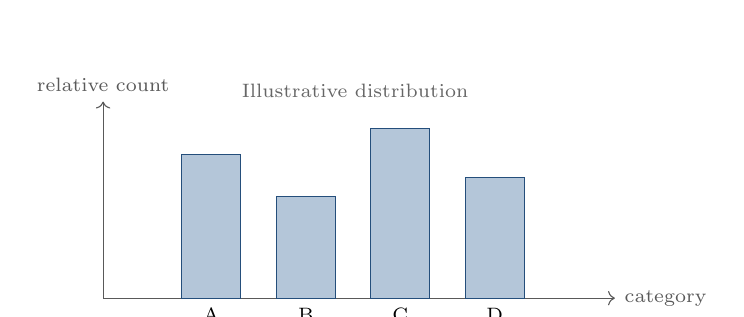
\begin{tikzpicture}[x=1cm,y=.48cm, font=\scriptsize]
      \draw[->,black!65] (0,0) -- (6.5,0) node[right] {category};
      \draw[->,black!65] (0,0) -- (0,5.2) node[above] {relative count};
      \foreach \x/\h/\t in {1/3.8/A,2.2/2.7/B,3.4/4.5/C,4.6/3.2/D}{
        \filldraw[fill=reportblue!35,draw=reportblue!85!black] (\x,0) rectangle +(0.75,\h);
        \node[below] at (\x+.375,0) {\t};
      }
      \node[align=center, text=black!60] at (3.2,5.5) {Illustrative distribution};
    \end{tikzpicture}
    \caption{#1}\label{#3}
  \end{figure}%
}

\newcounter{reportdiagram}
\newcommand{\ReportCommentFigure}{%
  \stepcounter{reportdiagram}%
  \ifcase\value{reportdiagram}\or
    \ReportFlow{Evolution of communication networks from conventional architectures to intelligent AI-driven 5G ecosystems.}{reportblue}{Conventional networks}{Cellular networks}{Software-defined networking}{Cloud-native 5G}{AI-driven ecosystems}{fig:network_evolution}%
  \or \ReportFlow{Overall internship workflow and engineering pipeline.}{reportblue}{Requirements study}{Mininet simulation}{RSNSD engineering}{SliceNet design}{Evaluation and roadmap}{fig:overall_workflow}%
  \or \ReportStack{Methodology adopted during the internship.}{reportblue}{Knowledge acquisition}{Simulation and hybrid data acquisition}{RSNSD dataset engineering}{SliceNet model development}{Experimental evaluation}{fig:methodology}%
  \or \ReportFlow{Evolution of mobile communication technologies from analog cellular systems to intelligent AI-enabled 5G networks.}{reportblue}{1G\\Analog voice}{2G\\Digital voice}{3G\\Mobile data}{4G\\Mobile broadband}{5G\\AI-enabled services}{fig:mobile_generations}%
  \or \ReportFlow{High-level architecture of a modern 5G communication network.}{reportblue}{User equipment}{Radio access network}{5G core\\control and user plane}{Edge and cloud services}{AI management and orchestration}{fig:5g_architecture}%
  \or \ReportFlow{Major functional entities within the 5G Core Network.}{reportblue}{User equipment}{gNodeB}{AMF / SMF\\control plane}{UPF\\user plane}{Data networks}{fig:5g_core}%
  \or \ReportFlow{Representative rural communication network deployment.}{reportgreen}{Rural users and IoT}{Local access network}{Private 5G RAN}{Local edge and 5G core}{Public and cloud services}{fig:rural_network}%
  \or \ReportFlow{Traditional 5G network slicing architecture over a shared physical infrastructure.}{reportorange}{Service requests}{eMBB slice}{URLLC slice}{mMTC slice}{Shared physical infrastructure}{fig:traditional_slicing}%
  \or \ReportFlow{Application-oriented service-aware network slicing framework.}{reportgreen}{Service traffic}{Service classification}{QoS and context mapping}{Logical service slices}{Shared 5G infrastructure}{fig:service_slicing}%
  \or \ReportFlow{AI-assisted network management workflow.}{reportblue}{Traffic monitoring}{Feature extraction}{AI inference}{Resource allocation}{Slice configuration}{fig:ai_networking}%
  \or \ReportFlow{Machine learning pipeline for traffic classification.}{reportblue}{Traffic flows}{Feature vectors}{Training data}{Classifier}{Service prediction}{fig:ml_pipeline}%
  \or \ReportFlow{Closed-loop self-healing network architecture.}{reportgreen}{Network telemetry}{Anomaly detection}{Diagnosis}{Recovery action}{Performance feedback}{fig:self_healing}%
  \or \ReportFlow{Limitations of conventional network management approaches.}{reportred}{Static policies}{Generic slice classes}{Limited rural data}{Manual optimisation}{Poor adaptability}{fig:current_limitations}%
  \or \ReportFlow{Motivation behind the proposed service-aware networking framework.}{reportorange}{5G applications}{Rural challenges}{Research gaps}{Simulation and RSNSD}{AI service model}{fig:research_motivation}%
  \or \ReportFlow{Engineering roadmap of the proposed project.}{reportblue}{Requirements study}{Simulation platform}{RSNSD engineering}{SliceNet perception}{Future autonomy}{fig:engineering_roadmap}%
  \or \ReportFlow{Overall project architecture for intelligent service-aware networking.}{reportblue}{Rural services}{Mininet simulation}{RSNSD dataset}{SliceNet classifier}{Intelligent orchestration}{fig:overall_architecture}%
  \or \ReportFlow{Experimental environment architecture.}{reportblue}{Service hosts}{Mininet topology}{Open vSwitch}{Traffic monitor}{Dataset storage}{fig:experimental_environment}%
  \or \ReportFlow{Mininet simulation architecture used during the internship.}{reportblue}{Traffic generators}{Mininet hosts}{Open vSwitch}{Controller}{Flow monitoring}{fig:simulation_architecture}%
  \or \ReportFlow{Rural Mininet topology.}{reportgreen}{Rural service hosts}{Access switch}{Aggregation switch}{Gateway}{External services}{fig:mininet_topology}%
  \or \ReportStack{Service-aware traffic generation pipeline.}{reportgreen}{Healthcare, education, agriculture and general-service profiles}{Traffic profile generator}{Packet generation}{Mininet transmission and monitoring}{Captured traffic for RSNSD}{fig:traffic_generation}%
  \or \ReportFlow{Feature extraction pipeline used for generating RSNSD.}{reportblue}{Captured packets}{Packet parsing}{Flow aggregation}{Feature computation}{RSNSD records}{fig:feature_pipeline}%
  \or \ReportFlow{Complete dataset generation workflow adopted during the internship.}{reportblue}{Mininet traffic}{Synthetic traffic}{Schema harmonisation}{Feature and label engineering}{RSNSD v1.0}{fig:dataset_pipeline}%
  \or \ReportFlow{Motivation for the Rural Service-aware Network Slice Dataset (RSNSD).}{reportorange}{Rural diversity}{QoS heterogeneity}{Dataset gap}{Hybrid data engineering}{RSNSD v1.0}{fig:dataset_motivation}%
  \or \ReportFlow{RSNSD generation pipeline.}{reportgreen}{Scenario definitions}{Simulation acquisition}{Synthetic generation}{Schema harmonisation}{Labeled RSNSD}{fig:rsnsd_pipeline}%
  \or \ReportFlow{Simulation-based data acquisition workflow.}{reportblue}{Scenario configuration}{Mininet execution}{Service traffic}{Flow capture}{Simulation samples}{fig:simulation_pipeline}%
  \or \ReportFlow{Synthetic data generation workflow.}{reportorange}{Statistical profiles}{Parameter sampling}{Synthetic flows}{Quality checks}{Synthetic samples}{fig:synthetic_pipeline}%
  \or \ReportFlow{Schema harmonisation pipeline for RSNSD.}{reportgreen}{Simulation schema}{Synthetic schema}{Field standardisation}{Validation}{Unified RSNSD schema}{fig:schema}%
  \or \ReportFlow{Scenario distribution represented in RSNSD.}{reportblue}{Normal operation}{High demand}{Congestion}{Emergency response}{Disaster recovery}{fig:scenario_distribution}%
  \or \ReportFlow{RSNSD feature engineering pipeline.}{reportblue}{Raw traffic}{Packet parsing}{Flow aggregation}{Feature validation}{Final feature vector}{fig:rsnsd_feature_engineering}%
  \or \ReportStack{Automatic label generation workflow for RSNSD.}{reportgreen}{Simulation configuration}{Service and scenario mapping}{QoS priority mapping}{Network slice mapping}{Labeled RSNSD record}{fig:label_generation}%
  \or \ReportStack{Dataset validation and quality-assurance workflow.}{reportblue}{Schema validation}{Completeness checks}{Range and consistency checks}{Class-balance assessment}{Validated RSNSD}{fig:validation}%
  \or \ReportBars{Simulation vs synthetic sample contribution.}{reportblue}{fig:source_distribution}%
  \or \ReportBars{Packet size distribution.}{reportblue}{fig:packet_distribution}%
  \or \ReportBars{Flow duration distribution.}{reportblue}{fig:flow_distribution}%
  \or \ReportBars{Bandwidth utilization across service categories.}{reportblue}{fig:bandwidth}%
  \or \ReportFlow{Position of SliceNet within the intelligent networking framework.}{reportblue}{Mininet simulation}{RSNSD v1.0}{SliceNet\\perception layer}{Context and slice selection}{Future RL and self-healing}{fig:slicenet_framework}%
  \or \ReportFlow{Service classification problem formulation adopted for SliceNet.}{reportblue}{Network flow}{Engineered feature vector}{Feature preprocessing}{SliceNet}{Service-class prediction}{fig:classification_problem}%
  \or \ReportStack{Feature preprocessing pipeline used before training SliceNet.}{reportblue}{Raw RSNSD features}{Missing-value and type checks}{Encoding categorical attributes}{Normalisation}{Model-ready feature vectors}{fig:feature_preprocessing}%
  \or \ReportFlow{Architecture of the proposed SliceNet neural network.}{reportblue}{Input features}{Dense layer + ReLU}{Batch norm + dropout}{Dense layer + ReLU}{Softmax service classes}{fig:slicenet_architecture}%
  \or \ReportStack{Training workflow adopted for SliceNet.}{reportblue}{RSNSD dataset}{Train, validation and test split}{Model optimisation}{Validation and tuning}{Final test evaluation}{fig:training_workflow}%
  \or \ReportFlow{Future evolution of the proposed intelligent networking framework beyond the internship.}{reportgreen}{SliceNet predictions}{Context engine}{Slice selection}{RL resource allocation}{Autonomous self-healing}{fig:future_pipeline}%
  \fi
}

% Emit an editable figure immediately before each existing commented specification,
% then preserve the specification itself as non-typeset source documentation.
\let\ReportOriginalComment\comment
% \begin{comment} opens a local group before it invokes \comment.  Schedule
% the figure after the original implementation closes that group; otherwise a
% float created here is discarded along with the commented material.
\renewcommand{\comment}{\aftergroup\ReportCommentFigure\ReportOriginalComment}


%==========================================
% Header
%==========================================

\pagestyle{fancy}

\fancyhf{}

\fancyhead[L]{Internship Training Report}

\fancyhead[R]{NITK Surathkal}

\fancyfoot[C]{\thepage}
\begin{document}

\begin{titlepage}
	
	\begin{center}
		
		\vspace*{1cm}
		
		{\Large \textbf{Practical Training REPORT}}
		
		\vspace{1.3cm}
		
		{\Large
			\textbf{CARS-SF: A Context-Aware Autonomous Rural Service Slicing Framework for Private 5G Networks}
		}
		
		\vspace{2cm}
		
		Submitted in partial fulfillment of the requirements\\
		for the Summer Internship
		
		\vspace{1.8cm}
		
		\textbf{Submitted By}
		
		\vspace{0.4cm}
		
		\textbf{Bammidi Ketan Rao}
		
		Roll No.: 252CS006
		
		Department of Computer Science and Engineering
		
		\vspace{1.8cm}
		
		
		\vfill
		
		
		\vspace{0.6cm}
		
		Department of Computer Science and Engineering
		
		National Institute of Technology Karnataka
		
		Surathkal -- 575025
		
		\vspace{0.8cm}
		
		Academic Year 2026--2027
		
	\end{center}
	
\end{titlepage}



	%%%%%%%%%%%%%%%%%%%%%%%%%%%%%%%%%%%%%%%%%%%%%%%%%%%%%%%%%%%%%
	%%%%%%%%%%%%%%%%%%%%%%%% ABSTRACT %%%%%%%%%%%%%%%%%%%%%%%%%%%
	%%%%%%%%%%%%%%%%%%%%%%%%%%%%%%%%%%%%%%%%%%%%%%%%%%%%%%%%%%%%%
	
\chapter*{Abstract}

Reliable communication infrastructure is essential for delivering critical services such as healthcare, education, agriculture, emergency response, and government applications in rural regions. However, conventional network management approaches are largely reactive and are unable to adapt efficiently to dynamic service demands, resource constraints, and network failures. These limitations motivate the development of intelligent network management frameworks capable of supporting service-aware communication and future autonomous operation.

This internship focused on establishing the engineering foundation for an Artificial Intelligence (AI)-driven network management framework for rural private 5G networks. The work began with an extensive study of private 5G architecture, network slicing, software-defined networking, virtualization technologies, and AI-assisted network management. Based on these studies, a Mininet-based simulation environment was developed to emulate realistic rural communication scenarios involving multiple service categories such as healthcare, education, agriculture, emergency services, government services, and general Internet traffic.

A hybrid traffic generation framework was subsequently designed to combine simulation-derived traffic with statistically generated synthetic traffic for comprehensive dataset engineering. Using this framework, the Rural Service-aware Network Slice Dataset (RSNSD) was developed with a unified feature schema, service-aware labels, and context-aware scenarios suitable for machine learning applications. In addition, the feasibility of an initial deep learning model, named SliceNet, was investigated as the first intelligent component of the proposed framework for service classification. Although full-scale model training and deployment remain part of the subsequent major project, the internship established the simulation infrastructure, dataset engineering pipeline, and AI development framework required for future work on intelligent network slicing, reinforcement learning-based resource allocation, failure prediction, and autonomous self-healing in rural private 5G networks.

\vspace{0.6cm}

\noindent\textbf{Keywords:}
Private 5G Networks,
Rural Communication Networks,
Network Slicing,
Artificial Intelligence,
Mininet,
RSNSD,
Service-aware Traffic,
Dataset Engineering,
SliceNet,
Autonomous Network Management.
	
	\clearpage
	
	
	%%%%%%%%%%%%%%%%%%%%%%%%%%%%%%%%%%%%%%%%%%%%%%%%%%%%%%%%%%%%%
	%%%%%%%%%%%%%%%% TABLE OF CONTENTS %%%%%%%%%%%%%%%%%%%%%%%%%%%
	%%%%%%%%%%%%%%%%%%%%%%%%%%%%%%%%%%%%%%%%%%%%%%%%%%%%%%%%%%%%%
	
	\clearpage
	\pagenumbering{roman}
	
	\tableofcontents
	\clearpage
	
	%%%%%%%%%%%%%%%%%%%%%%%%%%%%%%%%%%%%%%%%%%%%%%%%%%%%%%%%%%%%%
	%%%%%%%%%%%%%%%%%%% LIST OF FIGURES %%%%%%%%%%%%%%%%%%%%%%%%%%
	%%%%%%%%%%%%%%%%%%%%%%%%%%%%%%%%%%%%%%%%%%%%%%%%%%%%%%%%%%%%%
	
	\listoffigures
	\clearpage
	
	%%%%%%%%%%%%%%%%%%%%%%%%%%%%%%%%%%%%%%%%%%%%%%%%%%%%%%%%%%%%%
	%%%%%%%%%%%%%%%%%%%% LIST OF TABLES %%%%%%%%%%%%%%%%%%%%%%%%%%
	%%%%%%%%%%%%%%%%%%%%%%%%%%%%%%%%%%%%%%%%%%%%%%%%%%%%%%%%%%%%%
	
	\listoftables
	\clearpage
	
	%%%%%%%%%%%%%%%%%%%%%%%%%%%%%%%%%%%%%%%%%%%%%%%%%%%%%%%%%%%%%
	%%%%%%%%%%%%%%%%%%% MAIN CONTENT %%%%%%%%%%%%%%%%%%%%%%%%%%%%%
	%%%%%%%%%%%%%%%%%%%%%%%%%%%%%%%%%%%%%%%%%%%%%%%%%%%%%%%%%%%%%
	
	\pagenumbering{arabic}
	\setcounter{page}{1}
	
	\chapter{Introduction}
	\label{chap:introduction}
	
	The emergence of Fifth Generation (5G) communication networks has transformed modern digital connectivity by providing enhanced bandwidth, ultra-low latency, massive device connectivity, and flexible service provisioning. These capabilities have accelerated the adoption of intelligent applications across diverse domains, including healthcare, agriculture, education, industrial automation, emergency response, and smart governance. While considerable progress has been achieved in urban deployments, extending comparable communication services to rural and remote regions continues to present significant technical and operational challenges.
	
	Unlike urban environments, rural communication networks often operate under limited infrastructure availability, dynamic service demands, constrained network resources, and heterogeneous traffic patterns. Critical services such as telemedicine, smart agriculture, remote education, and emergency communications frequently compete for the same network resources, making efficient service differentiation and intelligent resource allocation essential for maintaining acceptable Quality of Service (QoS). Conventional network management approaches, which largely rely on static policies and manual configuration, are often inadequate for adapting to these continuously changing operating conditions.
	
	Recent advances in Artificial Intelligence (AI) and Machine Learning (ML) have demonstrated considerable potential for enabling intelligent and autonomous network management. By learning traffic characteristics, identifying service requirements, and supporting data-driven decision making, AI-based techniques provide the foundation for future context-aware network slicing, dynamic resource allocation, and autonomous self-healing communication systems. However, the effectiveness of such techniques is fundamentally dependent on the availability of representative datasets and realistic simulation environments that accurately capture the operational characteristics of rural communication networks.
	
	Motivated by these challenges, the internship focused on establishing the initial engineering foundation for an AI-driven service-aware networking framework. The work involved the development of a Mininet-based simulation environment capable of emulating rural communication scenarios, the engineering of the Rural Service-aware Network Slice Dataset (RSNSD) through a hybrid simulation and synthetic data generation pipeline, and the implementation of an initial deep learning model, SliceNet, for service classification. Collectively, these components establish the first stage of a larger research effort towards intelligent network slicing and autonomous self-healing 5G communication networks.
	
	This chapter presents the motivation for the internship, outlines the research problem and objectives, summarizes the scope of work and key deliverables, and provides an overview of the organization of the report.
	
	
	%=============================================================================
	\section{Motivation}
	\label{sec:motivation}
	
	%----------------------------------------------------
	% Figure 1.1
	%----------------------------------------------------
	\begin{comment}
	\begin{figure}[H]
		\centering
		%\includegraphics[width=0.9\textwidth]{figures/architecture/5g_evolution.pdf}
		\fbox{\rule{0pt}{2.5in}\rule{0.9\textwidth}{0pt}}
		\caption{Evolution of communication networks from conventional architectures
			to intelligent AI-driven 5G ecosystems.}
		\label{fig:network_evolution}
	\end{figure}
	\end{comment}
	
	The evolution of mobile communication networks has been driven by the continuous demand for higher data rates, improved reliability, and support for increasingly diverse applications. Each successive generation of mobile technology has introduced significant advancements in network capability, beginning with analog voice communication in First Generation (1G) networks, followed by digital communication in Second Generation (2G), mobile internet access in Third Generation (3G), broadband connectivity in Fourth Generation (4G), and highly flexible, software-driven communication infrastructures in Fifth Generation (5G) networks.
	
	Unlike previous generations, 5G extends beyond improvements in communication speed and capacity by introducing virtualization, software-defined networking, network function virtualization, and network slicing. These technologies enable communication networks to dynamically allocate resources based on application requirements rather than relying on static infrastructure configurations. Consequently, modern communication systems are capable of simultaneously supporting heterogeneous services with vastly different Quality of Service (QoS) requirements.
	
	The growing diversity of applications has also increased the complexity of network management. Critical services such as remote healthcare, disaster response, precision agriculture, and smart education require reliable and context-aware resource allocation that conventional rule-based management approaches cannot efficiently provide. As network scale and complexity continue to increase, manual configuration and static policy enforcement become increasingly inadequate for ensuring efficient utilization of available resources.
	
	Artificial Intelligence (AI) has therefore emerged as a promising technology for enabling autonomous network management. By continuously analyzing network traffic, learning service characteristics, predicting future demands, and assisting resource allocation decisions, AI enables communication networks to transition from reactive operation toward proactive and intelligent management. This evolution forms the fundamental motivation behind the present internship, which focuses on developing the initial components required for an AI-assisted service-aware networking framework through realistic simulation, dataset engineering, and machine learning-based service classification.
	
	
	%=============================================================================
	\section{Research Gap}
	\label{sec:problem_overview}
	
	%----------------------------------------------------
	% Table 1.1
	%----------------------------------------------------
	
	\begin{table}[H]
		\centering
		\caption{Major Challenges in Rural Communication Networks}
		\label{tab:rural_challenges}
		
		\begin{tabular}{|p{4cm}|p{9cm}|}
			\hline
			
			\textbf{Challenge} &
			\textbf{Description}
			\\
			\hline
			
			Limited Network Infrastructure &
			Rural deployments often operate with fewer base stations, limited backhaul capacity, and constrained computational resources, resulting in reduced network coverage and service availability.
			\\
			\hline
			
			Heterogeneous Service Requirements &
			Applications such as telemedicine, precision agriculture, remote education, emergency response, and general Internet access exhibit significantly different Quality of Service (QoS) requirements, making uniform resource allocation ineffective.
			\\
			\hline
			
			Lack of Representative Datasets &
			Publicly available network traffic datasets rarely capture service-aware rural communication scenarios, limiting the development and evaluation of AI-driven network management solutions.
			\\
			\hline
			
			Static Network Management &
			Conventional network management techniques rely on predefined rules and manual configuration, making them unsuitable for adapting to rapidly changing traffic patterns and dynamic service demands.
			\\
			\hline
			
		\end{tabular}
		
	\end{table}
	
	The challenges summarized in Table~\ref{tab:rural_challenges} collectively demonstrate that efficient rural communication extends beyond simply providing network connectivity. Instead, modern rural networks must intelligently recognize the nature of ongoing communication, prioritize critical services, and dynamically allocate limited resources according to changing operational contexts. Addressing these challenges requires an integrated engineering approach combining realistic network simulation, representative dataset generation, and artificial intelligence-based traffic understanding.
	
	The internship was therefore designed to establish the initial components of such a framework. A Mininet-based simulation environment was developed to emulate representative rural communication scenarios, while the Rural Service-aware Network Slice Dataset (RSNSD) was engineered to provide training data for intelligent networking applications. Building upon this dataset, an initial deep learning model, SliceNet, was developed to classify service categories from network traffic, thereby establishing the perception layer for future context-aware network slicing and autonomous self-healing mechanisms.
	
	%=============================================================================
	\section{Internship Objectives}
	\label{sec:objectives}
	
	The primary objectives of the internship are summarized as follows:
	
	\begin{enumerate}
		
		\item To study the architecture, operational principles, and resource management mechanisms of modern Fifth Generation (5G) communication networks with emphasis on rural deployment scenarios.
		
		\item To design and implement a Mininet-based simulation environment capable of emulating service-aware rural communication networks under multiple operational scenarios.
		
		\item To develop a hybrid data acquisition pipeline by integrating simulation-generated traffic with synthetic traffic generation techniques for creating representative network datasets.
		
		\item To engineer the Rural Service-aware Network Slice Dataset (RSNSD) through feature extraction, schema design, data harmonization, and automated labeling methodologies.
		
		\item To develop and evaluate an initial deep learning-based service classification model, SliceNet, capable of identifying service categories from network traffic flows.
		
		\item To establish the engineering foundation for future context-aware network slicing, reinforcement learning-based resource allocation, and autonomous self-healing network management.
		
	\end{enumerate}
	
	
	%=============================================================================
	\section{Scope of Work}
	\label{sec:scope}
	
	The scope of the internship was centered on establishing the initial engineering foundation for an AI-assisted service-aware network management framework targeted towards rural communication networks. Rather than developing a complete autonomous networking solution, the internship focused on constructing the core components required to support future research on intelligent network slicing, reinforcement learning-based resource allocation, and autonomous self-healing mechanisms.
	
	The work carried out during the internship encompassed the following major activities:
	
	\begin{itemize}
		
		\item Conducting a comprehensive study of modern 5G communication networks, private 5G deployments, network slicing, and artificial intelligence techniques used in network management.
		
		\item Designing and implementing a Mininet-based simulation environment capable of emulating representative rural communication scenarios under different service contexts.
		
		\item Developing a hybrid data acquisition framework by combining simulation-generated traffic with statistically generated synthetic traffic to improve dataset diversity and coverage.
		
		\item Engineering the Rural Service-aware Network Slice Dataset (RSNSD), including feature extraction, schema design, data harmonization, automated labeling, and dataset validation.
		
		\item Designing, implementing, and evaluating an initial deep learning model, SliceNet, for service classification using the engineered dataset.
		
		\item Performing experimental evaluation of the simulation framework, dataset, and classification model using quantitative performance metrics and visualization techniques.
		
	\end{itemize}
	
	The scope of the internship was intentionally limited to the development of the simulation environment, dataset engineering pipeline, and initial artificial intelligence model. Advanced components such as reinforcement learning-based scheduling, dynamic network slice orchestration, failure prediction, and autonomous self-healing mechanisms are identified as future extensions of this work and form part of the ongoing research roadmap presented in Chapter~\ref{chap:conclusion}.
	
	
	%----------------------------------------------------
	% Figure 1.2
	%----------------------------------------------------
	\begin{comment}
	\begin{figure}[H]
		\centering
		%\includegraphics[width=0.9\textwidth]{figures/architecture/workflow.pdf}
		\fbox{\rule{0pt}{3in}\rule{0.85\textwidth}{0pt}}
		\caption{Overall internship workflow and engineering pipeline.}
		\label{fig:overall_workflow}
	\end{figure}
	content...
\end{comment}
	
	%=============================================================================
	\section{Internship Deliverables}
	\label{sec:deliverables}
	
	%----------------------------------------------------
	% Table 1.2
	%----------------------------------------------------
	
	\begin{table}[H]
		\centering
		\caption{Summary of Internship Deliverables}
		\label{tab:deliverables}
		
		\begin{tabular}{|c|p{4cm}|p{8cm}|}
			\hline
			
			\textbf{ID} &
			\textbf{Deliverable} &
			\textbf{Description} \\
			\hline
			
			D1 &
			Simulation Framework &
			Development of a Mininet-based simulation environment capable of emulating service-aware rural communication networks under multiple operational scenarios. \\
			\hline
			
			D2 &
			Hybrid Data Acquisition Pipeline &
			Implementation of a unified data generation framework combining simulation-derived traffic with synthetic traffic generation techniques to improve dataset diversity and coverage. \\
			\hline
			
			D3 &
			RSNSD v1.0 Dataset &
			Engineering of the Rural Service-aware Network Slice Dataset (RSNSD), including feature extraction, schema harmonization, automated labeling, and dataset validation. \\
			\hline
			
			D4 &
			SliceNet v1.0 &
			Development of an initial deep learning-based service classification model capable of identifying rural service categories from network traffic flows. \\
			\hline
			
			D5 &
			Experimental Evaluation Framework &
			Performance evaluation of the simulation environment, engineered dataset, and SliceNet model using quantitative metrics and visualization techniques. \\
			\hline
			
		\end{tabular}
		
	\end{table}

	
	%=============================================================================
	\section{Methodology Overview}
	\label{sec:methodology}
	
	%----------------------------------------------------
	% Figure 1.3
	%----------------------------------------------------
					\begin{comment}
	\begin{figure}[H]
		\centering
		\fbox{
			\parbox[c][4.5in][c]{0.92\textwidth}{
				\centering
				\Large\textbf{Placeholder: Methodology Workflow Diagram}\\[0.5cm]
				
				\normalsize
				
				\textbf{Expected Structure}

				\begin{enumerate}
					\item Phase I -- Knowledge Acquisition
					\begin{itemize}
						\item Literature Review
						\item Problem Identification
					\end{itemize}
					
					\item Phase II -- Simulation Engineering
					\begin{itemize}
						\item Mininet-based Simulation
						\item Synthetic Traffic Generation
						\item Hybrid Data Acquisition
					\end{itemize}
					
					\item Phase III -- Dataset Engineering
					\begin{itemize}
						\item RSNSD v1.0 Construction
						\item Feature Engineering
						\item Schema Harmonization
						\item Automatic Labeling
					\end{itemize}
					
					\item Phase IV -- AI Model Development
					\begin{itemize}
						\item SliceNet v1.0
						\item Training
						\item Validation
						\item Testing
					\end{itemize}
					
					\item Phase V -- Experimental Evaluation
					\begin{itemize}
						\item Performance Analysis
						\item Visualization
						\item Engineering Observations
						\item Future Research Roadmap
					\end{itemize}
				\end{enumerate}
				
				\textbf{Diagram Requirements}
				\begin{itemize}
					\item Five sequential engineering phases.
					\item Top-to-bottom workflow.
					\item Directed arrows indicating data flow.
					\item Mininet and Synthetic Generator merge into Hybrid Data Acquisition.
					\item Professional IEEE thesis style.
					\item Rounded rectangular blocks with minimal color.
					\item Suitable for vector recreation in TikZ.
				\end{itemize}
			}

		}
		
		\caption{Methodology adopted during the internship.}
		\label{fig:methodology}
	\end{figure}
			\end{comment}
	
	Figure~\ref{fig:methodology} presents the overall methodology adopted during the internship. The work commenced with a detailed study of modern 5G communication systems, network slicing, and artificial intelligence techniques applicable to network management. Based on the identified research gap, representative rural communication scenarios were designed to capture the diverse service requirements expected in real-world deployments.
	
	To generate representative training data, two complementary data acquisition strategies were employed. The first strategy utilized a Mininet-based simulation framework to emulate realistic network traffic under multiple operational scenarios, while the second strategy employed statistically guided synthetic data generation to improve dataset diversity and coverage. The outputs from both acquisition pipelines were harmonized into a unified dataset schema, resulting in the Rural Service-aware Network Slice Dataset (RSNSD v1.0).
	
	Following dataset construction, feature engineering techniques were applied to extract meaningful representations of network traffic suitable for machine learning applications. The engineered dataset was subsequently used to develop SliceNet v1.0, an initial deep learning model capable of classifying network flows according to their corresponding service categories. Finally, the simulation framework, dataset, and classification model were evaluated using quantitative performance metrics and visualization techniques, providing valuable engineering insights that establish the foundation for future work on context-aware network slicing, reinforcement learning-based resource allocation, and autonomous self-healing communication systems.
	
	


	
	%%%%%%%%%%%%%%%%%%%%%%%%%%%%%%%%%%%%%%%%%%%%%%%%%%%%%%%%%%%%%%%%%%%%%%%%%%%%%%
	% Chapter 2
	%%%%%%%%%%%%%%%%%%%%%%%%%%%%%%%%%%%%%%%%%%%%%%%%%%%%%%%%%%%%%%%%%%%%%%%%%%%%%%
	
	\chapter{Literature Study}
	\label{chap:background}
	
	The realization of intelligent and autonomous communication networks relies on the integration of advanced mobile networking technologies, network virtualization, artificial intelligence, and data-driven decision-making techniques. Recent developments in Fifth Generation (5G) communication systems have introduced capabilities such as network slicing, software-defined networking, and cloud-native network functions, enabling communication infrastructures to dynamically support heterogeneous services with diverse Quality of Service (QoS) requirements. These advancements have created new opportunities for applying artificial intelligence to automate network monitoring, resource management, and service orchestration.
	
	The internship presented in this report builds upon these emerging technologies to establish the initial engineering foundation for an AI-assisted service-aware network management framework. Accordingly, a clear understanding of the underlying communication architecture, intelligent networking concepts, simulation environments, and machine learning techniques is essential for motivating the design decisions described in the subsequent chapters.
	
	This chapter reviews the theoretical concepts that underpin the internship. It introduces the architecture and characteristics of modern 5G communication networks, discusses the principles of network slicing and service-aware communication, presents the role of artificial intelligence in network management, and reviews the simulation and machine learning concepts that motivated the development of the Mininet-based simulation framework, the Rural Service-aware Network Slice Dataset (RSNSD), and the SliceNet service classification model.
	
	
	%=============================================================================
	\section{Evolution of Mobile Communication Networks}
	\label{sec:evolution}
	
The evolution of mobile communication networks has been driven by the continuous demand for improved connectivity, higher data rates, lower latency, and support for an increasingly diverse range of communication services. Successive generations of mobile technology have progressively enhanced network capabilities, transforming wireless communication from basic voice connectivity into a versatile platform capable of supporting broadband, multimedia, and machine-to-machine communication.

The first generation (1G) introduced analog cellular voice communication, while the second generation (2G) transitioned to digital communication technologies with support for voice, SMS, and basic data services. Third generation (3G) networks enabled mobile Internet access and multimedia applications, whereas Fourth Generation (4G) Long-Term Evolution (LTE) networks significantly improved bandwidth, latency, and all-IP connectivity, facilitating the widespread adoption of cloud services, high-definition video streaming, and mobile broadband applications.

Fifth Generation (5G) represents a fundamental architectural evolution~\cite{shafi20175g, chataut2020massive} rather than merely an increase in communication speed. By incorporating technologies such as Software Defined Networking (SDN)~\cite{kreutz2015software, mckeown2008openflow}, Network Function Virtualization (NFV), cloud-native architectures, and network slicing, 5G enables communication resources to be dynamically managed according to application requirements. This programmable and service-oriented architecture establishes the technological foundation for intelligent communication systems discussed in the subsequent sections. Figure~\ref{fig:mobile_generations} illustrates the evolution of mobile communication technologies from early analog systems to modern software-driven 5G networks.

	
	%----------------------------------------------------
	% Figure 2.1
	%----------------------------------------------------
\begin{comment}
	\begin{figure}[H]
		\centering
		\fbox{
			\parbox[c][4.5in][c]{0.92\textwidth}{
				\centering
				\Large\textbf{Placeholder: Evolution of Mobile Communication Networks}\\[0.6cm]
				
				\textbf{Figure Objective}
				
				Illustrate the technological evolution from first-generation
				mobile communication systems to modern intelligent 5G networks,
				highlighting the progressive improvements in communication
				capabilities and the emergence of AI-assisted network management.
				
				\vspace{0.5cm}
				
				\textbf{Timeline Structure}
				
				\begin{enumerate}
					\item 1G -- Analog Voice Communication
					\item 2G -- Digital Voice and SMS
					\item 3G -- Mobile Internet and Multimedia
					\item 4G -- Broadband IP Networks
					\item 5G -- Network Slicing, SDN, NFV, Edge Computing
					\item AI-enabled 5G -- Intelligent Resource Allocation,
					Service Awareness, Autonomous Network Management
				\end{enumerate}
				
				\vspace{0.5cm}
				
				\textbf{Visual Requirements}
				
				\begin{itemize}
					\item Horizontal chronological timeline.
					\item Six generations represented using equally spaced nodes.
					\item Progressive increase in capability from left to right.
					\item Distinct visual emphasis on 5G and AI-enabled networking.
					\item Modern IEEE-style infographic.
					\item Minimal color palette with vector graphics.
					\item Suitable for recreation using TikZ or Figma.
				\end{itemize}
			}
		}
		
		\caption{Evolution of mobile communication technologies from analog cellular systems to intelligent AI-enabled 5G communication networks.}
		\label{fig:mobile_generations}
		
	\end{figure}
\end{comment}
	
	%----------------------------------------------------
	% Table 2.1
	%----------------------------------------------------
	
	\begin{table}[H]
		\centering
		\caption{Comparison of Mobile Communication Generations}
		\label{tab:mobile_generations}
		
		\begin{tabular}{|c|c|p{3cm}|p{2.5cm}|p{5cm}|}
			\hline
			
			\textbf{Generation} &
			\textbf{Year} &
			\textbf{Technology} &
			\textbf{Peak Speed} &
			\textbf{Typical Applications}
			\\
			\hline
			
			1G &
			1980s &
			Analog Cellular &
			$\sim$2.4 kbps &
			Voice communication
			\\
			\hline
			
			2G &
			1990s &
			GSM, CDMA &
			$\sim$64 kbps &
			Digital voice, SMS, basic data services
			\\
			\hline
			
			3G &
			2000s &
			UMTS, HSPA &
			Up to 2 Mbps &
			Mobile Internet, multimedia, video calling
			\\
			\hline
			
			4G &
			2010s &
			LTE, LTE-Advanced &
			Up to 1 Gbps &
			HD video streaming, cloud services, mobile broadband
			\\
			\hline
			
			5G &
			2020s &
			5G NR &
			Up to 20 Gbps &
			Network slicing, IoT, autonomous systems, edge computing, AI-assisted network management
			\\
			\hline
			
		\end{tabular}
		
	\end{table}
	
	%=============================================================================
	\section{Fifth Generation (5G) Networks}
	\label{sec:5g}
	
	Fifth Generation (5G) communication networks represent a major advancement in mobile networking by introducing a flexible, software-driven architecture capable of supporting a wide variety of communication services. Unlike previous generations, which primarily focused on improving communication speed and capacity, 5G provides a unified platform for enhanced Mobile Broadband (eMBB), massive Machine-Type Communication (mMTC), and Ultra-Reliable Low-Latency Communication (URLLC). These capabilities enable the deployment of diverse applications across domains such as healthcare, transportation, agriculture, industrial automation, and smart cities.
	
	A distinguishing feature of 5G is its service-oriented architecture, which separates network functionality into modular and virtualized components. Technologies including Software Defined Networking (SDN), Network Function Virtualization (NFV), Multi-access Edge Computing (MEC), and cloud-native network functions enable communication services to be deployed, scaled, and managed dynamically. This architectural flexibility improves resource utilization, simplifies network management, and provides the foundation for highly programmable communication infrastructures.
	
	In addition to virtualization, 5G introduces support for network slicing, enabling multiple logical networks to operate independently over a shared physical infrastructure while satisfying different Quality of Service (QoS) requirements. These capabilities make 5G significantly more adaptable than previous generations and establish the technological foundation for intelligent communication systems discussed in the subsequent sections. Figure~\ref{fig:5g_architecture} presents a high-level view of the major functional components of a modern 5G communication network.
	
\begin{figure}
	\centering
	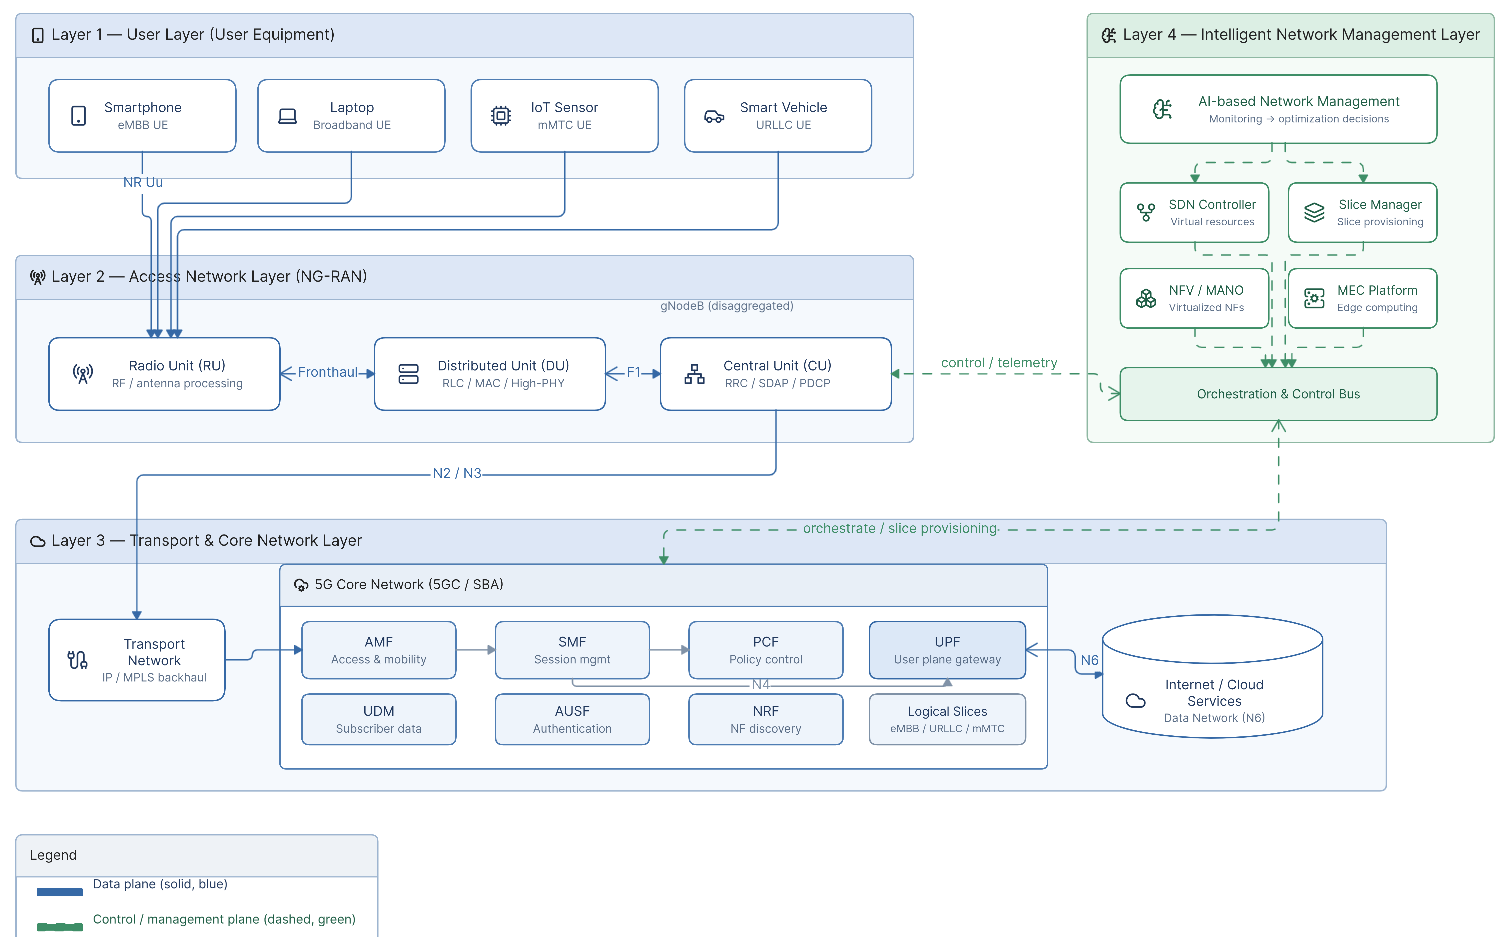
\includegraphics[width=0.8\linewidth]{screenshot003}
	\caption{High-level architecture of a modern 5G communication network highlighting the major functional components and intelligent management framework.}
	\label{fig:5g_architecture}
\end{figure}
	
	%=============================================================================
	\subsection{5G Core Network}
	
	The Fifth Generation Core Network (5GC) provides the control and data management functions required to support communication services in modern 5G systems. Unlike previous generations, the 5GC adopts a Service-Based Architecture (SBA) in which network functions operate as modular and virtualized services that communicate through standardized interfaces. This cloud-native architecture improves scalability, flexibility, and resource utilization while enabling rapid deployment of new communication services. The separation of control-plane and user-plane functions further enhances network efficiency by allowing independent management of signaling and user traffic.
	
	The 5GC comprises several specialized Network Functions (NFs), each responsible for a specific aspect of network operation. The Access and Mobility Management Function (AMF) manages device registration, authentication, and mobility, while the Session Management Function (SMF) establishes and controls communication sessions. User data is forwarded through the User Plane Function (UPF), whereas the Policy Control Function (PCF) enforces Quality of Service (QoS) and network policies. Additional functions such as the Unified Data Management (UDM), Authentication Server Function (AUSF), and Network Repository Function (NRF) support subscriber management, authentication, and service discovery. Together, these network functions provide the flexible and programmable core infrastructure required for intelligent communication networks.
	%----------------------------------------------------
	% Figure 2.3
	%----------------------------------------------------
	
	
	%----------------------------------------------------
	% Table 2.2
	%----------------------------------------------------
	
	\begin{table}[H]
		\centering
		\caption{Functions of Major 5G Core Network Components}
		\label{tab:5gc_components}
		
		\begin{tabular}{|p{3cm}|p{10cm}|}
			\hline
			
			\textbf{Component} &
			\textbf{Primary Function}
			\\
			\hline
			
			Access and Mobility Management Function (AMF) &
			Manages user registration, authentication procedures, mobility management, connection establishment, and access control between User Equipment (UE) and the 5G Core Network.
			\\
			\hline
			
			Session Management Function (SMF) &
			Establishes, modifies, and terminates communication sessions while allocating IP addresses, managing Quality of Service (QoS), and controlling user-plane resources.
			\\
			\hline
			
			User Plane Function (UPF) &
			Handles packet forwarding, traffic routing, packet inspection, Quality of Service (QoS) enforcement, and communication between the 5G Core and external data networks.
			\\
			\hline
			
			Unified Data Management (UDM) &
			Maintains subscriber profiles, authentication credentials, service subscriptions, and user-related information required by network functions.
			\\
			\hline
			
			Authentication Server Function (AUSF) &
			Performs user authentication and security verification before allowing access to network services.
			\\
			\hline
			
			Policy Control Function (PCF) &
			Generates policy rules governing Quality of Service (QoS), charging, session management, and service-specific resource allocation.
			\\
			\hline
			
			Network Slice Selection Function (NSSF) &
			Selects appropriate network slices for individual users and services based on subscription information, service requirements, and network policies.
			\\
			\hline
			
		\end{tabular}
		
	\end{table}
	
	%=============================================================================
\subsection{Radio Access Network}

The Radio Access Network (RAN) forms the interface between User Equipment (UE) and the 5G Core Network, providing wireless connectivity and managing radio resources. In Fifth Generation (5G) networks, the traditional base station is replaced by the Next Generation NodeB (gNodeB or gNB), which is responsible for radio transmission, mobility management, scheduling, and forwarding user traffic to the core network. The gNodeB is logically divided into three functional components: the Radio Unit (RU), the Distributed Unit (DU), and the Central Unit (CU), enabling flexible deployment and scalable network architectures.

\begin{figure}[H]
	\centering
	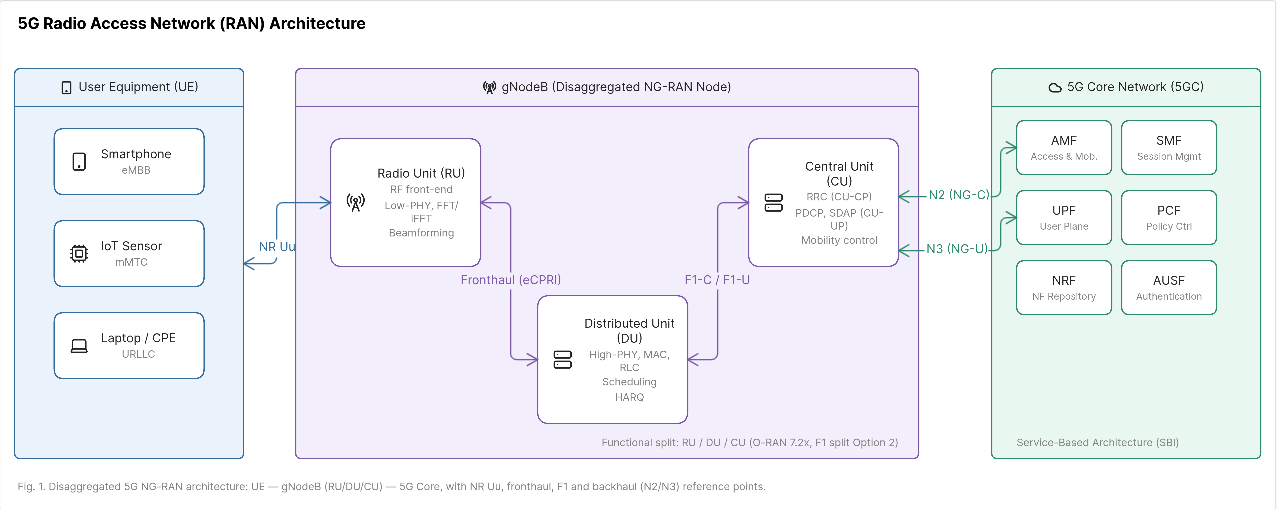
\includegraphics[width=\textwidth]{screenshot001}
	\caption{5G Radio Access Network (RAN) architecture.}
	\label{fig:ran}
\end{figure}

The User Equipment communicates with the Radio Unit through the New Radio (NR) air interface. The Radio Unit performs radio frequency transmission and reception, the Distributed Unit executes real-time baseband processing, and the Central Unit manages higher-layer protocol functions before forwarding traffic to the 5G Core Network. These functional units are interconnected through fronthaul, midhaul, and backhaul transport networks, allowing operators to distribute processing resources efficiently while supporting high-capacity, low-latency communication services. Figure~\ref{fig:ran} illustrates the high-level architecture of the 5G Radio Access Network.

%==================================================================
	\section{Private 5G Networks}
	\label{sec:private5g}
	
	Private Fifth Generation (5G) networks are dedicated communication infrastructures deployed and managed by individual organizations to provide secure, reliable, and customizable wireless connectivity within a defined geographical area. Unlike public cellular networks operated by commercial telecom providers, private 5G networks are designed to satisfy the specific communication requirements of enterprises, industrial facilities, healthcare organizations, research institutions, university campuses, and rural communities. By providing exclusive access to network resources, private deployments offer greater control over network operation, security, and service quality.
	
	A typical private 5G deployment consists of a localized Radio Access Network (RAN), an independent or locally deployed 5G Core Network (5GC), and dedicated computing and networking infrastructure. This architecture enables organizations to configure Quality of Service (QoS) policies, security mechanisms, and service provisioning according to application-specific requirements. Such flexibility allows communication resources to be optimized for mission-critical services while ensuring efficient utilization of the available infrastructure.
	
	Private 5G networks are particularly well suited for environments where communication requirements vary significantly across applications, such as rural communities, industrial facilities, and research testbeds. Their programmable architecture supports customized network management, service differentiation, and application-specific resource allocation, making them an attractive platform for developing and evaluating advanced communication technologies.
	
	
	%----------------------------------------------------
	% Table 2.3
	%----------------------------------------------------
	
	\begin{table}[H]
		\centering
		\caption{Comparison Between Public and Private 5G Networks}
		\label{tab:private5g}
		
		\begin{tabular}{|p{3.8cm}|p{5.2cm}|p{5.2cm}|}
			\hline
			
			\textbf{Aspect} &
			\textbf{Public 5G} &
			\textbf{Private 5G}
			\\
			\hline
			
			Ownership &
			Owned and operated by commercial telecom service providers. &
			Owned and managed by an enterprise, institution, or organization.
			\\
			\hline
			
			Coverage Area &
			Wide-area coverage serving cities, regions, and nationwide deployments. &
			Localized coverage such as factories, campuses, hospitals, or rural communities.
			\\
			\hline
			
			Infrastructure &
			Shared among a large number of subscribers and applications. &
			Dedicated infrastructure reserved for a specific organization or use case.
			\\
			\hline
			
			Network Control &
			Configuration and management are controlled by the network operator. &
			Complete administrative control over network configuration, policies, and services.
			\\
			\hline
			
			Quality of Service (QoS) &
			Resources are shared among users, resulting in varying service quality. &
			QoS policies can be customized to satisfy application-specific requirements.
			\\
			\hline
			
			Security &
			Security policies are defined by the public network operator. &
			Enhanced security through isolated infrastructure and organization-specific policies.
			\\
			\hline
			
			Network Slicing &
			Limited user-level customization of network slices. &
			Network slices can be designed and optimized for organization-specific services.
			\\
			\hline
			
			Typical Applications &
			Consumer mobile broadband, voice services, and public Internet access. &
			Industrial automation, healthcare, smart agriculture, research laboratories, university campuses, and mission-critical communications.
			\\
			\hline
			
		\end{tabular}
		
	\end{table}
	
	%=============================================================================
	\section{Rural Communication Networks}
	\label{sec:rural}
	
Rural communication networks play a crucial role in extending digital connectivity to geographically dispersed communities where conventional communication infrastructure is often limited. Reliable communication services enable applications such as telemedicine, precision agriculture, remote education, digital governance, and disaster response, thereby contributing to social and economic development. As broadband connectivity continues to expand into underserved regions, rural communication networks have become an increasingly important area of research and industrial innovation.

Unlike urban deployments, rural communication networks are characterized by sparse population density, large geographical coverage, limited infrastructure availability, and constrained computational resources. Communication resources must therefore be shared among applications with diverse Quality of Service (QoS) requirements, ranging from latency-sensitive healthcare and emergency services to bandwidth-intensive education and best-effort Internet access. Traditional rule-based resource management strategies often struggle to adapt efficiently to these heterogeneous and dynamically changing service demands, resulting in suboptimal resource utilization and inconsistent service quality.

Artificial Intelligence (AI) and Machine Learning (ML) offer promising solutions for addressing these challenges by enabling communication networks to monitor traffic patterns, identify service characteristics, and support intelligent resource allocation. Motivated by this vision, the internship focuses on developing the foundational engineering components required for service-aware rural communication networks, including a realistic Mininet-based simulation environment, the Rural Service-aware Network Slice Dataset (RSNSD), and the SliceNet service classification model. Together, these components establish the data and perception layer necessary for future intelligent network slicing and autonomous network management.

	

	%=============================================================================
	\section{Network Slicing}
	\label{sec:slicing}
	
Network slicing is one of the defining capabilities of Fifth Generation (5G) communication networks, enabling multiple logical networks, or \emph{network slices}, to operate independently over a shared physical infrastructure. Each slice is configured to satisfy specific Quality of Service (QoS) requirements, such as bandwidth, latency, reliability, and security, allowing heterogeneous applications to coexist without compromising performance. Unlike traditional communication networks that apply uniform resource management policies to all traffic, network slicing enables communication resources to be allocated according to application-specific requirements. This flexibility is achieved through enabling technologies such as Software Defined Networking (SDN), Network Function Virtualization (NFV), and cloud-native architectures, which allow network functions and services to be dynamically deployed and managed.

Despite its flexibility, efficient resource allocation across multiple network slices remains a challenging task due to continuously changing traffic demands and service priorities. Artificial Intelligence (AI) and Machine Learning (ML) techniques have therefore emerged as promising solutions for intelligent slice management by analyzing network traffic, identifying service requirements, and supporting context-aware resource allocation. The internship presented in this report contributes towards this vision by developing the foundational engineering components required for AI-assisted network slicing, including a Mininet-based simulation framework, the Rural Service-aware Network Slice Dataset (RSNSD), and the SliceNet service classification model. Together, these components establish the perception layer required for future intelligent scheduling and autonomous network orchestration.
.
	

	
\begin{table}[H]
	\centering
	\caption{Comparison of Standard 5G Network Slice Categories}
	\label{tab:slices}
	
	\begin{tabular}{|p{2.5cm}|p{5.5cm}|p{6cm}|}
		\hline
		
		\textbf{Slice} &
		\textbf{Key Characteristics} &
		\textbf{Representative Applications}
		\\
		\hline
		
		Enhanced Mobile Broadband (eMBB) &
		High bandwidth, high throughput, moderate latency, optimized for data-intensive applications. &
		Ultra-HD video streaming, virtual reality (VR), augmented reality (AR), cloud gaming, high-speed mobile Internet.
		\\
		\hline
		
		Ultra-Reliable Low-Latency Communication (URLLC) &
		Ultra-low latency, extremely high reliability, deterministic communication for mission-critical services. &
		Industrial automation, autonomous vehicles, remote surgery, smart grids, emergency communications.
		\\
		\hline
		
		Massive Machine-Type Communication (mMTC) &
		Supports a very large number of low-power devices with infrequent data transmission and high energy efficiency. &
		Internet of Things (IoT), smart agriculture, environmental monitoring, smart metering, asset tracking.
		\\
		\hline
		
	\end{tabular}
	
\end{table}
	
	%=============================================================================
	\subsection{Service-Aware Network Slicing}
	
Traditional network slicing categorizes communication services into three broad classes: enhanced Mobile Broadband (eMBB), Ultra-Reliable Low-Latency Communication (URLLC), and massive Machine-Type Communication (mMTC). While this classification is well suited for general-purpose 5G deployments, it does not adequately capture the diverse application requirements of private rural communication networks. Services such as healthcare, education, agriculture, emergency response, and government applications exhibit distinct operational priorities that extend beyond the conventional 3GPP slice taxonomy. Consequently, allocating network resources solely on the basis of standard slice categories may not achieve optimal resource utilization or service quality.

Service-aware network slicing addresses this limitation by classifying traffic according to application domains and allocating network resources based on the specific Quality of Service (QoS) requirements of each service. The internship presented in this report adopts this application-oriented approach by considering service classes including healthcare, education, agriculture, emergency services, government services, industrial IoT, and general Internet traffic. These service categories form the foundation of the Rural Service-aware Network Slice Dataset (RSNSD) and provide the contextual information required for future AI-assisted network slicing and autonomous resource management.

	
	
	%----------------------------------------------------
	% Table 2.5
	%----------------------------------------------------
	
\begin{table}[H]
	\centering
	\caption{Primary Service Classes Considered in this Work}
	\label{tab:services}
	
	\begin{tabular}{|p{4cm}|p{9cm}|}
		\hline
		
		\textbf{Service Class} &
		\textbf{Description}
		\\
		\hline
		
		Healthcare &
		Telemedicine, remote patient monitoring, medical consultations, and healthcare applications requiring reliable and low-latency communication.
		\\
		\hline
		
		Education &
		Remote classrooms, online learning platforms, digital libraries, and educational content delivery services.
		\\
		\hline
		
		Agriculture &
		Precision farming, environmental sensing, smart irrigation, crop monitoring, and agricultural IoT applications.
		\\
		\hline
		
		General Communication &
		Conventional Internet access, web browsing, multimedia streaming, messaging, and other best-effort communication services.
		\\
		\hline
		
	\end{tabular}
	
\end{table}
	
	%=============================================================================
	\section{Artificial Intelligence in Network Management}
	\label{sec:ai}
	
Artificial Intelligence (AI) has become an essential component of modern communication network management due to the increasing complexity of 5G infrastructures. Contemporary networks must support heterogeneous applications, dynamic traffic patterns, and diverse Quality of Service (QoS) requirements while adapting to continuously changing network conditions. Traditional rule-based management approaches often struggle to meet these demands, leading to inefficient resource utilization and increased operational complexity. AI techniques enable communication networks to analyze historical and real-time network data, identify traffic patterns, classify application services, predict network behavior, and assist in intelligent resource allocation. These capabilities support advanced functionalities such as network slicing, anomaly detection, predictive maintenance, and autonomous network optimization.

The internship presented in this report focuses on establishing the initial perception layer required for AI-assisted network management rather than implementing a complete autonomous networking framework. The work includes the development of a realistic simulation environment, the Rural Service-aware Network Slice Dataset (RSNSD), and the SliceNet service classification model, which together provide the data generation, feature engineering, and traffic classification capabilities necessary for future reinforcement learning-based resource allocation and intelligent network slicing.

	

	%----------------------------------------------------
	% Table 2.6
	%----------------------------------------------------
	
	\begin{table}[H]
		\centering
		\caption{Applications of Artificial Intelligence in Communication Networks}
		\label{tab:ai_networking}
		
		\begin{tabular}{|p{5cm}|p{8cm}|}
			\hline
			
			\textbf{Application} &
			\textbf{Description}
			\\
			\hline
			
			Traffic Classification &
			Machine learning models automatically identify network traffic according to application or service type, enabling service-aware communication and intelligent resource management.
			\\
			\hline
			
			Resource Allocation &
			AI algorithms dynamically allocate network bandwidth, computing resources, and Quality of Service (QoS) parameters based on changing traffic conditions and service priorities.
			\\
			\hline
			
			Network Slice Management &
			Artificial Intelligence assists in selecting, configuring, and optimizing network slices to satisfy the requirements of heterogeneous communication services.
			\\
			\hline
			
			Anomaly and Fault Detection &
			Learning-based techniques continuously monitor network behaviour to identify abnormal traffic patterns, failures, security threats, and performance degradation.
			\\
			\hline
			
			Predictive Network Maintenance &
			Historical network data is analyzed to predict potential failures, enabling proactive maintenance and reducing service interruptions.
			\\
			\hline
			
			Autonomous Network Management &
			AI supports closed-loop network operation by continuously monitoring network conditions, making intelligent decisions, executing corrective actions, and learning from previous outcomes.
			\\
			\hline
			
		\end{tabular}
		
	\end{table}
	
	%=============================================================================
	\section{Machine Learning for Traffic Classification}
	\label{sec:traffic_classification}
	
	Network traffic classification is the process of identifying the application or service associated with a communication flow by analyzing its observable characteristics. Traditional classification techniques relied on port numbers and deep packet inspection; however, these approaches have become less effective due to encrypted communication, dynamic port allocation, and the growing diversity of Internet applications. Consequently, machine learning techniques have emerged as an effective alternative by learning traffic patterns directly from network features rather than relying on predefined rules.
	
	A typical machine learning pipeline for traffic classification consists~\cite{nguyen2008survey, pacheco2018machine, wang2015end} of traffic collection, feature extraction, data preprocessing, model training, and performance evaluation. Network flow statistics, packet-level characteristics, and temporal features are commonly used as input to supervised learning algorithms for service identification. The work presented in this internship follows this general workflow by engineering the Rural Service-aware Network Slice Dataset (RSNSD) and utilizing it to develop SliceNet, an initial deep learning model for service-aware traffic classification.
	
	\begin{comment}
		\begin{figure}[H]
			\centering
			\fbox{
				\parbox[c][4.3in][c]{0.92\textwidth}{
					
					\centering
					\Large\textbf{Placeholder: Machine Learning Pipeline for Traffic Classification}
					
					\vspace{0.5cm}
					
					\textbf{Pipeline}
					
					\begin{center}
						Traffic Collection
						$\rightarrow$
						Feature Extraction
						$\rightarrow$
						Data Preprocessing
						$\rightarrow$
						Model Training
						$\rightarrow$
						Prediction
						$\rightarrow$
						Performance Evaluation
					\end{center}
					
					\vspace{0.4cm}
					
					\textbf{Visual Requirements}
					
					\begin{itemize}
						\item Left-to-right pipeline.
						\item Six sequential processing stages.
						\item Data flows represented using arrows.
						\item Minimal IEEE-style vector diagram.
					\end{itemize}
					
				}
			}
			
			\caption{General machine learning pipeline for network traffic classification.}
			\label{fig:ml_pipeline}
			
		\end{figure}
	\end{comment}
	
	%=============================================================================
	\section{Self-Healing Networks}
	\label{sec:self_healing}
	
	Self-healing communication networks are intelligent systems capable of automatically detecting network anomalies, identifying their root causes, selecting appropriate recovery strategies, and restoring normal operation with minimal human intervention. By integrating continuous network monitoring with artificial intelligence and automated control mechanisms, self-healing networks improve service availability, reduce operational overhead, and enhance overall network resilience. These capabilities are particularly valuable in modern communication systems where network conditions change dynamically and service continuity is essential.
	
	Most self-healing frameworks follow a closed-loop control architecture consisting of four major stages: monitoring, analysis, decision-making, and execution. Network telemetry is continuously collected and analyzed to detect abnormal conditions, after which intelligent algorithms determine suitable recovery actions that are automatically applied to the network. Although the internship presented in this report does not implement a complete self-healing framework, it establishes the perception layer required for future autonomous operation through realistic network simulation, service-aware dataset engineering, and machine learning-based traffic classification.

	%----------------------------------------------------
	% Table 2.7
	%----------------------------------------------------
	
	\begin{table}[H]
		\centering
		\caption{Simulation and Development Tools Used During the Internship}
		\label{tab:simulation_tools}
		
		\begin{tabular}{|p{4cm}|p{9cm}|}
			\hline
			
			\textbf{Tool} &
			\textbf{Purpose}
			\\
			\hline
			
			Mininet &
			Emulation of service-aware rural communication networks, network topologies, traffic flows, and resource allocation scenarios used for dataset generation.
			\\
			\hline
			
			Open vSwitch (OVS) &
			Implementation of programmable virtual switches for packet forwarding, traffic isolation, and software-defined networking experiments within the Mininet environment.
			\\
			\hline
			
			Python &
			Development of simulation scripts, synthetic traffic generators, feature extraction modules, dataset engineering pipeline, and machine learning workflows.
			\\
			\hline
			
			Pandas and NumPy &
			Data preprocessing, feature engineering, statistical analysis, dataset validation, and preparation of the Rural Service-aware Network Slice Dataset (RSNSD).
			\\
			\hline
			
			PyTorch &
			Implementation, training, validation, and evaluation of the SliceNet deep learning model for service-aware network traffic classification.
			\\
			\hline
			
			Git and GitHub &
			Version control, source code management, collaborative development, and maintenance of the simulation framework and associated software modules.
			\\
			\hline
			
		\end{tabular}
		
	\end{table}
	
	\begin{table}[H]
		\centering
		\caption{Research Gap and Motivation for the Proposed Work}
		\label{tab:research_gap}
		
		\begin{tabular}{|p{6.2cm}|p{6.2cm}|}
			\hline
			
			\textbf{Existing Limitation} &
			\textbf{Motivation for This Work}
			\\
			\hline
			
			Most existing studies focus on urban communication environments with high infrastructure density. &
			Develop a simulation framework representative of rural communication networks with heterogeneous service requirements and limited infrastructure.
			\\
			\hline
			
			Publicly available network traffic datasets rarely capture service-aware rural communication scenarios. &
			Develop the Rural Service-aware Network Slice Dataset (RSNSD) using a hybrid simulation and synthetic data generation pipeline.
			\\
			\hline
			
			Conventional network slicing primarily follows generic 3GPP slice categories (eMBB, URLLC, and mMTC). &
			Investigate application-oriented service classes such as healthcare, education, agriculture, emergency services, government services, industrial IoT, and general Internet traffic.
			\\
			\hline
			
			Traditional resource allocation approaches rely heavily on static rules and manual configuration. &
			Establish the perception layer required for future AI-assisted and context-aware network slicing through service classification.
			\\
			\hline
			
			Few existing studies provide an end-to-end engineering workflow connecting simulation, dataset generation, and machine learning for rural private 5G networks. &
			Develop an integrated engineering framework combining network simulation, dataset engineering, and an initial deep learning-based service classification model.
			\\
			\hline
			
		\end{tabular}
		
	\end{table}
	%=============================================================================

This chapter presented the theoretical foundations necessary for understanding the engineering work undertaken during the internship, including the evolution of mobile communication networks, 5G architecture, private 5G deployments, rural communication networks, network slicing, and the role of Artificial Intelligence (AI) in modern network management. The discussion also highlighted the limitations of existing approaches and the need for intelligent, service-aware, and data-driven communication systems, thereby establishing the motivation for the research problem and engineering methodology presented in the following chapter.


	%%%%%%%%%%%%%%%%%%%%%%%%%%%%%%%%%%%%%%%%%%%%%%%%%%%%%%%%%%%%%%%%%%%%%%%%%%%%%%
	% Chapter 3
	%%%%%%%%%%%%%%%%%%%%%%%%%%%%%%%%%%%%%%%%%%%%%%%%%%%%%%%%%%%%%%%%%%%%%%%%%%%%%%
	
	\chapter{Project Definition}
	\label{chap:problem_statement}
	
	The background concepts presented in the previous chapter highlight the opportunities offered by modern 5G communication networks as well as the challenges associated with intelligent network management in rural environments. Building upon these foundations, this chapter formulates the research problem addressed during the internship, defines the project objectives, identifies the system requirements, and outlines the engineering methodology adopted for the design and implementation of the proposed framework.
	
	\section{Problem Statement}
	\label{sec:problem_statement}
	
	Modern 5G communication networks are expected to support a diverse range of applications with significantly different Quality of Service (QoS) requirements while operating over a common physical infrastructure. Although network slicing provides the flexibility to allocate resources according to service demands, existing network management approaches predominantly rely on predefined policies and standardized slice categories. Such methods are often inadequate for rural communication environments, where heterogeneous services, limited infrastructure, and dynamically changing traffic patterns demand more adaptive and context-aware resource management strategies.
	
	Existing publicly available network traffic datasets primarily focus on problems such as intrusion detection, Quality of Service prediction, or generic traffic classification, with limited consideration for application-oriented rural communication scenarios. Similarly, conventional network slicing frameworks largely follow the standard 3GPP categories of enhanced Mobile Broadband (eMBB), Ultra-Reliable Low-Latency Communication (URLLC), and massive Machine-Type Communication (mMTC), which do not explicitly capture the service diversity encountered in rural deployments. Consequently, current approaches provide limited support for understanding application-specific communication behaviour in service-aware private 5G networks.
	
	These limitations highlight the need for an engineering framework capable of generating representative rural communication data, identifying application-specific service characteristics, and establishing the perception layer required for intelligent network management. Addressing these challenges forms the primary motivation for the work carried out during this internship and serves as the foundation for the engineering methodology presented in the subsequent sections.
	
	\begin{comment}
		content...\begin{figure}[H]
			\centering
			\fbox{
				\parbox[c][4.8in][c]{0.92\textwidth}{
					
					\centering
					\Large\textbf{Placeholder: Limitations of Conventional Network Management}
					
					\vspace{0.5cm}
					
					\textbf{Objective}
					
					Illustrate the shortcomings of traditional network management
					approaches when applied to rural private 5G communication
					environments.
					
					\vspace{0.4cm}
					
					\textbf{Major Limitations}
					
					\begin{itemize}
						\item Static rule-based resource allocation
						\item Generic eMBB/URLLC/mMTC slice categories
						\item Lack of rural service-aware datasets
						\item Limited context awareness
						\item Manual network optimization
						\item Poor adaptability to dynamic traffic conditions
					\end{itemize}
					
					\vspace{0.4cm}
					
					\textbf{Visual Requirements}
					
					\begin{itemize}
						\item Left: Conventional network management
						\item Right: List of resulting challenges
						\item Red callout boxes highlighting limitations
						\item IEEE-style conceptual illustration
					\end{itemize}
					
				}
			}
			
			\caption{Limitations of conventional network management approaches.}
			
			\label{fig:current_limitations}
			
		\end{figure}
	\end{comment}
	
	\section{Project Objectives}
	\label{sec:research_objectives}
	
	\subsection{Primary Objective}
	
	The primary objective of this internship is to develop the foundational engineering components of an AI-assisted service-aware network management framework for rural private 5G communication networks by establishing a realistic simulation environment, engineering a representative service-aware dataset, and developing an initial machine learning model for network traffic classification.
	
	\subsection{Secondary Objectives}
	
	To achieve the primary objective, the following secondary objectives were identified:
	
	\begin{itemize}
		
		\item Design and implement a Mininet-based simulation platform capable of emulating representative rural communication scenarios.
		
		\item Develop a hybrid data generation pipeline combining simulated and synthetic network traffic.
		
		\item Engineer the Rural Service-aware Network Slice Dataset (RSNSD) through feature extraction, preprocessing, and service-aware labeling.
		
		\item Develop and evaluate SliceNet, an initial deep learning model for service-aware network traffic classification.
		
		\item Establish a modular engineering framework that can support future research on intelligent network slicing, reinforcement learning-based resource allocation, and autonomous network management.
		
	\end{itemize}
	
	
	%----------------------------------------------------
	% Table 3.1
	%----------------------------------------------------
	
	\begin{table}[H]
		\centering
		\caption{Summary of Project Objectives}
		\label{tab:objectives}
		
		\begin{tabular}{|c|p{11cm}|}
			\hline
			
			\textbf{Objective} &
			\textbf{Description}
			\\
			\hline
			
			\textbf{O1} &
			Design and implement a Mininet-based simulation platform capable of emulating representative rural private 5G communication scenarios~\cite{yaacoub2020key, suomalainen20185g, chih2014toward}.
			\\
			\hline
			
			\textbf{O2} &
			Develop a hybrid data generation pipeline by integrating simulation-derived and synthetic network traffic for comprehensive dataset creation.
			\\
			\hline
			
			\textbf{O3} &
			Engineer the Rural Service-aware Network Slice Dataset (RSNSD) through feature extraction, preprocessing, schema design, and service-aware labeling.
			\\
			\hline
			
			\textbf{O4} &
			Develop and evaluate SliceNet, an initial deep learning model for service-aware network traffic classification.
			\\
			\hline
			
			\textbf{O5} &
			Establish a modular engineering framework that supports future research on intelligent network slicing, reinforcement learning-based resource allocation, and autonomous network management.
			\\
			\hline
			
		\end{tabular}
		
	\end{table}
	%=============================================================================
	\section{System Requirements}
	\label{sec:requirements}
	
	The proposed engineering framework was designed to satisfy a set of functional and non-functional requirements identified during the planning phase of the internship. These requirements guided the development of the simulation platform, dataset generation pipeline, and machine learning framework while ensuring modularity, reproducibility, and extensibility for future phases of the major project.
	\begin{table}[H]
		\centering
		\caption{Functional Requirements}
		\label{tab:functional_requirements}
		
		\begin{tabular}{|c|p{10.5cm}|}
			\hline
			
			\textbf{ID} &
			\textbf{Requirement}
			\\
			\hline
			
			FR1 &
			The system shall simulate representative rural communication network topologies.
			\\
			\hline
			
			FR2 &
			The system shall generate realistic service-aware network traffic under multiple operating scenarios.
			\\
			\hline
			
			FR3 &
			The system shall extract and preprocess network traffic features for dataset generation.
			\\
			\hline
			
			FR4 &
			The system shall automatically label generated traffic according to predefined service classes.
			\\
			\hline
			
			FR5 &
			The system shall train and evaluate a machine learning model for service-aware traffic classification.
			\\
			\hline
			
		\end{tabular}
		
	\end{table}
	
	\begin{table}[H]
		\centering
		\caption{Non-Functional Requirements}
		\label{tab:nonfunctional_requirements}
		
		\begin{tabular}{|c|p{10.5cm}|}
			\hline
			
			\textbf{ID} &
			\textbf{Requirement}
			\\
			\hline
			
			NFR1 &
			The framework shall be modular and extensible.
			\\
			\hline
			
			NFR2 &
			The implementation shall be reproducible across different development environments.
			\\
			\hline
			
			NFR3 &
			The framework shall support scalable dataset generation.
			\\
			\hline
			
			NFR4 &
			The implementation shall facilitate future integration of intelligent resource allocation modules.
			\\
			\hline
			
			NFR5 &
			The framework shall maintain a clear separation between simulation, dataset engineering, and machine learning components.
			\\
			\hline
			
		\end{tabular}
		
	\end{table}
	
	%=============================================================================
	\section{Engineering Roadmap}
	\label{sec:roadmap}
	
	The internship was executed through a structured engineering workflow comprising successive phases of system planning, simulation development, dataset engineering, and machine learning model development. Each phase builds upon the outputs of the previous stage, resulting in a modular and reproducible framework that serves as the foundation for subsequent phases of the major project.
	
	\begin{comment}
		\begin{figure}[H]
			\centering
			\fbox{
				\parbox[c][5.0in][c]{0.92\textwidth}{
					
					\centering
					\Large\textbf{Placeholder: Engineering Roadmap}
					
					\vspace{0.5cm}
					
					\textbf{Objective}
					
					Illustrate the phased engineering workflow adopted during the
					internship from problem definition to initial AI model development.
					
					\vspace{0.4cm}
					
					\textbf{Engineering Phases}
					
					\begin{enumerate}
						\item Problem Definition
						\item Requirement Analysis
						\item Simulation Platform Development
						\item Hybrid Traffic Generation
						\item Dataset Engineering (RSNSD)
						\item Machine Learning Model Development (SliceNet)
						\item Performance Evaluation
						\item Future Project Roadmap
					\end{enumerate}
					
					\vspace{0.4cm}
					
					\textbf{Visual Requirements}
					
					\begin{itemize}
						\item Horizontal timeline or left-to-right pipeline.
						\item Each phase represented by a process block.
						\item Arrows indicating sequential progression.
						\item Completed internship phases highlighted differently from future work.
						\item Professional IEEE-style vector illustration.
					\end{itemize}
					
				}
			}
			
			\caption{Engineering roadmap adopted during the internship.}
			
			\label{fig:engineering_roadmap}
			
		\end{figure}
	\end{comment}


	\section{Project Architecture}
	\label{sec:project_architecture}
	
	The engineering framework developed during the internship follows a modular pipeline in which each component performs a distinct function while contributing to the overall system workflow. The process begins with realistic rural network simulation and traffic generation, followed by dataset engineering and feature extraction, which provide the input for machine learning-based service classification. The outputs of these components establish the engineering foundation for future intelligent network slicing and autonomous network management. Figure~\ref{fig:overall_architecture} presents the high-level architecture of the complete internship framework.
	
\begin{figure}[H]
	\centering
	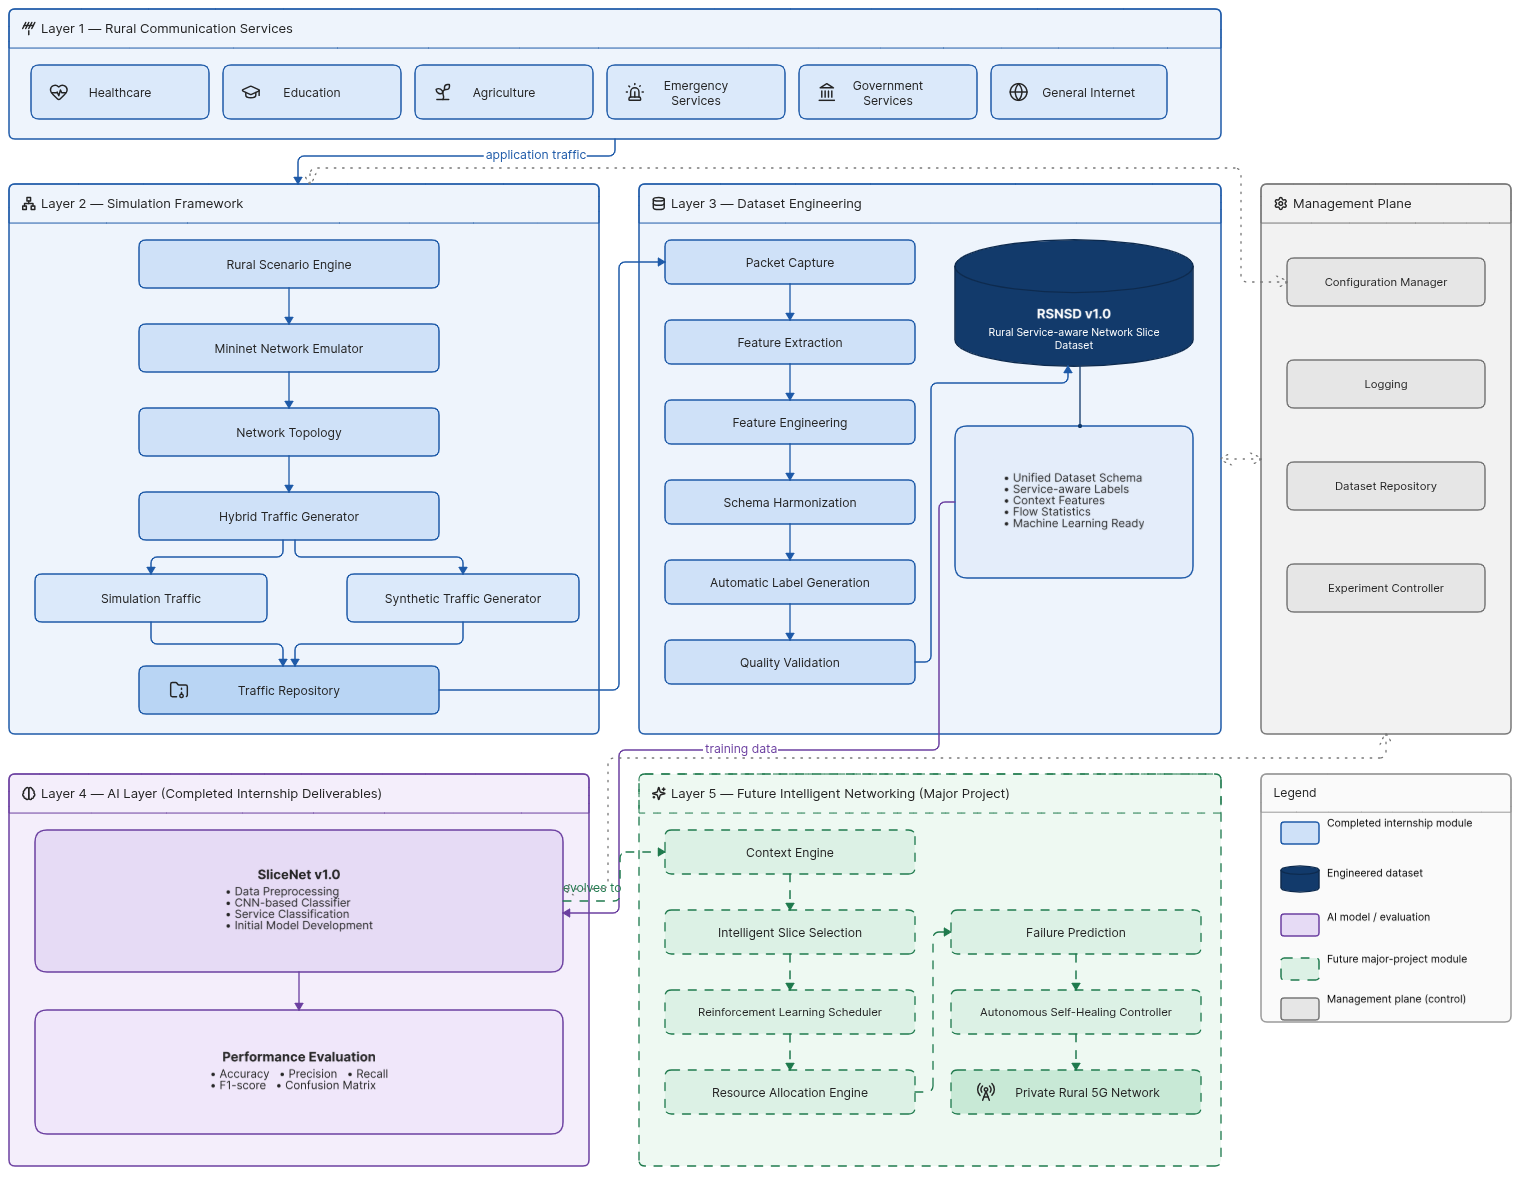
\includegraphics[
	width=\textwidth,
	height=.8\textheight,
	]{screenshot005}
	\caption{Overall architecture of the engineering framework.}
	\label{fig:overall_architecture}
\end{figure}
		

	%%%%%%%%%%%%%%%%%%%%%%%%%%%%%%%%%%%%%%%%%%%%%%%%%%%%%%%%%%%%%%%%%%%%%%%%%%%%%%
	% Chapter 4
	%%%%%%%%%%%%%%%%%%%%%%%%%%%%%%%%%%%%%%%%%%%%%%%%%%%%%%%%%%%%%%%%%%%%%%%%%%%%%%
	
	\chapter{System Design and Experimental Environment}
	\label{chap:experimental_environment}
	
	This chapter describes the experimental environment developed during the internship to support the implementation and evaluation of the proposed engineering framework. The environment was designed to emulate representative rural private 5G communication scenarios~\cite{yaacoub2020key, suomalainen20185g, chih2014toward} and generate service-aware network traffic for dataset engineering and machine learning applications. It comprises the software stack, network simulation platform, traffic generation framework, feature engineering pipeline, and the overall experimental workflow adopted throughout the internship.
	
	\section{System Overview}
	\label{sec:system_overview}
	
	The experimental environment follows a modular architecture in which individual components perform specific tasks while collectively supporting the end-to-end engineering workflow. The process begins with configurable rural communication scenarios that are executed within a Mininet-based simulation environment to generate representative network traffic. The generated traffic is subsequently processed through feature extraction and preprocessing modules before being organized into the Rural Service-aware Network Slice Dataset (RSNSD), which serves as the input for the SliceNet service classification model.
	
	The modular organization of the framework enables independent development, testing, and evaluation of each subsystem while maintaining a well-defined data flow between components. Such an architecture improves maintainability, simplifies experimentation, and provides flexibility for integrating additional modules in future phases of the major project.
	
	
	\begin{comment}
		\begin{figure}[H]
			\centering
			\fbox{
				\parbox[c][5.5in][c]{0.92\textwidth}{
					
					\centering
					\Large\textbf{Placeholder: Experimental Environment Architecture}
					
					\vspace{0.5cm}
					
					\textbf{Objective}
					
					Illustrate the overall software architecture of the experimental
					environment developed during the internship.
					
					\vspace{0.4cm}
					
					\textbf{Architecture Layers}
					
					\begin{enumerate}
						
						\item User Configuration Layer
						
						\item Rural Scenario Configuration
						
						\item Mininet Simulation Engine
						
						\item Traffic Generation Module
						
						\item Feature Extraction & Preprocessing
						
						\item RSNSD Dataset Repository
						
						\item SliceNet Classification Engine
						
						\item Evaluation & Visualization Module
						
					\end{enumerate}
					
					\vspace{0.4cm}
					
					\textbf{Visual Requirements}
					
					\begin{itemize}
						
						\item Layered architecture
						
						\item Downward data flow
						
						\item Dataset represented as a storage cylinder
						
						\item AI model represented as a rounded processing block
						
						\item IEEE publication quality
						
					\end{itemize}
					
				}
			}
			
			\caption{Overall architecture of the experimental environment.}
			
			\label{fig:system_overview}
			
		\end{figure}
	\end{comment}
	
	\section{Hardware Configuration}
	\label{sec:hardware}
	
	The development, simulation, and machine learning experiments conducted during the internship were performed on a single workstation configured to support the complete engineering workflow. The hardware configuration was sufficient for executing the Mininet-based simulation environment, dataset engineering pipeline, and the initial deep learning model development. Table~\ref{tab:hardware} summarizes the hardware and software specifications of the experimental platform.
	
	\begin{table}[H]
		\centering
		\caption{Hardware and Software Configuration of the Experimental Platform}
		\label{tab:hardware}
		
		\begin{tabular}{|p{5cm}|p{8cm}|}
			\hline
			
			\textbf{Component} &
			\textbf{Specification}
			\\
			\hline
			
			Processor &
			Intel Core i5 11th Generation Processor
			\\
			\hline
			
			CPU Cores &
			4 Cores / 8 Threads
			\\
			\hline
			
			Main Memory &
			16 GB DDR4 RAM
			\\
			\hline
			
			Storage &
			512 GB NVMe Solid State Drive (SSD)
			\\
			\hline
			
			Graphics &
			Integrated Intel Iris Xe Graphics
			\\
			\hline
			
			Operating System &
			Linux Mint 22.1 (64-bit)
			\\
			\hline
			
			Python Version &
			Python 3.12
			\\
			\hline
			
			Development Environment &
			Visual Studio Code
			\\
			\hline
			
			Version Control &
			Git and GitHub
			\\
			\hline
			
		\end{tabular}
		
	\end{table}
	
	
\section{Software Stack}
\label{sec:software_stack}

The implementation of the proposed engineering framework relied on a collection of open-source software tools and libraries for network simulation, data processing, machine learning, and visualization. These tools collectively supported the development of the simulation environment, dataset engineering pipeline, and traffic classification model. Table~\ref{tab:software} summarizes the primary software components used during the internship.

\begin{table}[H]
	\centering
	\caption{Software Stack Used During the Internship}
	\label{tab:software}
	
	\begin{tabular}{|p{3.5cm}|p{3cm}|p{8cm}|}
		\hline
		
		\textbf{Software} &
		\textbf{Version} &
		\textbf{Purpose}
		\\
		\hline
		
		Linux Mint &
		22.1 &
		Operating system for development and experimentation.
		\\
		\hline
		
		Python &
		3.12 &
		Primary programming language used for simulation, data processing, and machine learning.
		\\
		\hline
		
		Mininet &
		2.3.0 &
		Network emulation platform for constructing and evaluating rural communication scenarios.
		\\
		\hline
		
		Open vSwitch &
		System Package &
		Software-defined virtual switch used by Mininet to emulate network forwarding behaviour.
		\\
		\hline
		
		Scapy &
		Latest Stable &
		Packet generation and network traffic manipulation.
		\\
		\hline
		
		Pandas &
		Latest Stable &
		Dataset manipulation, preprocessing, and analysis.
		\\
		\hline
		
		NumPy &
		Latest Stable &
		Numerical computation and array processing.
		\\
		\hline
		
		NetworkX &
		Latest Stable &
		Network topology construction and graph-based analysis.
		\\
		\hline
		
		Matplotlib &
		Latest Stable &
		Performance visualization and experimental result plotting.
		\\
		\hline
		
		PyTorch &
		Latest Stable &
		Development and training of the SliceNet deep learning model.
		\\
		\hline
		
		Visual Studio Code &
		Latest Stable &
		Integrated development environment for implementation and debugging.
		\\
		\hline
		
		Git &
		Latest Stable &
		Version control and source code management.
		\\
		\hline
		
	\end{tabular}
	
\end{table}

	
\section{Simulation Architecture}
\label{sec:simulation_architecture}

The simulation architecture developed during the internship provides a configurable environment for emulating representative rural private 5G communication scenarios~\cite{yaacoub2020key, suomalainen20185g, chih2014toward}. Built upon the Mininet network emulator~\cite{lantz2010network, kaur2014mininet}, the framework models network entities such as hosts, switches, and communication links while allowing multiple application-specific service scenarios to be executed under controlled conditions. This enables the generation of realistic network traffic corresponding to different operational contexts without requiring dedicated physical networking infrastructure.

The simulation workflow follows a modular pipeline in which network scenarios are first configured and instantiated within Mininet, after which application traffic is generated and monitored to collect flow-level statistics. The captured traffic is subsequently processed through feature extraction and preprocessing modules before being forwarded to the dataset engineering pipeline. This modular design enables repeatable experimentation, simplifies the introduction of new service scenarios, and supports the systematic generation of representative data for subsequent machine learning applications.

\begin{figure}[H]
	\centering
	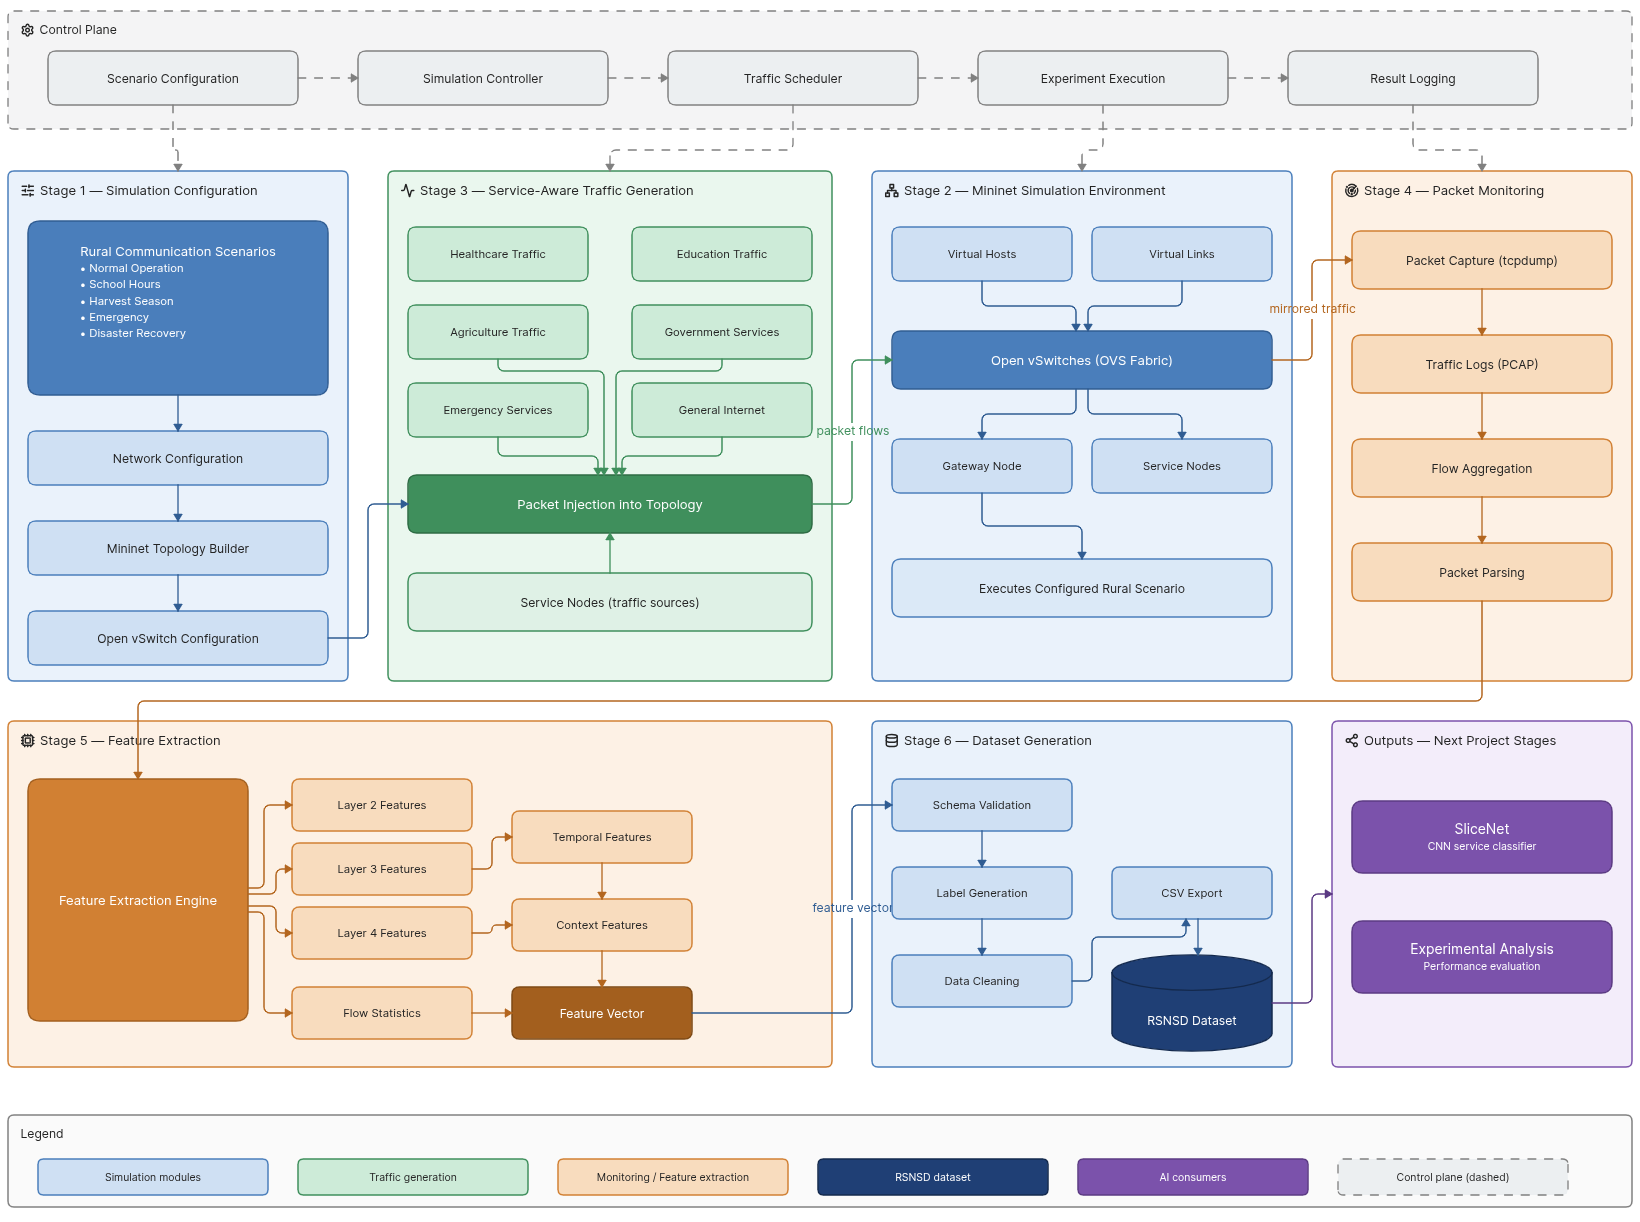
\includegraphics[
	width=\textwidth,
	height=0.68\textheight,
	]{screenshot006}
	\caption{Architecture of the Mininet-based traffic generation framework showing the complete data flow from rural communication scenarios to the RSNSD dataset.}
	\label{fig:simulation_workflow}
\end{figure}
	
\section{Mininet Topology}
\label{sec:mininet_topology}

The proposed simulation environment models a representative rural private 5G communication network using the Mininet network emulator~\cite{lantz2010network, kaur2014mininet}. The topology was designed to emulate a small-scale rural deployment in which multiple application services share a common communication infrastructure while exhibiting different traffic characteristics. The network consists of interconnected software-defined switches, end hosts representing service endpoints, and communication links configured to emulate realistic network connectivity under controlled experimental conditions.

Each host within the topology represents a specific application or service operating in the rural environment, while Open vSwitch instances emulate the forwarding behaviour~\cite{mckeown2008openflow} of network switches. Communication links interconnect these components to facilitate end-to-end traffic generation across the network. The modular design of the topology enables the introduction of multiple service scenarios by varying traffic patterns, communication endpoints, and network parameters without modifying the underlying network structure. This flexibility allows the same simulation environment to support healthcare, education, agriculture, and general communication workloads.

The topology was intentionally designed to be configurable and extensible, allowing additional hosts, switches, and service nodes to be incorporated as the major project evolves. Such a modular architecture simplifies experimentation, supports repeatable evaluations, and provides a realistic platform for generating representative network traffic for dataset engineering and machine learning applications.


	%----------------------------------------------------
	% Table 4.3
	%----------------------------------------------------
	\begin{table}[H]
		\centering
		\caption{Components of the Mininet Simulation Topology}
		\label{tab:topology}
		
		\begin{tabular}{|p{4cm}|p{2.5cm}|p{8cm}|}
			\hline
			
			\textbf{Component} &
			\textbf{Quantity} &
			\textbf{Description}
			\\
			\hline
			
			Core Switch &
			1 &
			Central Open vSwitch instance responsible for interconnecting all communication nodes.
			\\
			\hline
			
			Access Switches &
			Configurable &
			Software-defined switches connecting service hosts to the simulated communication network.
			\\
			\hline
			
			Service Hosts &
			Configurable &
			End hosts representing application-specific communication services such as healthcare, education, agriculture, and general communication.
			\\
			\hline
			
			Communication Links &
			Configurable &
			Virtual Ethernet links interconnecting hosts and switches with configurable network parameters.
			\\
			\hline
			
			SDN Controller &
			1 &
			Controller responsible for managing Open vSwitch forwarding behaviour within the Mininet environment.
			\\
			\hline
			
			Monitoring Node &
			1 &
			Collects traffic statistics and flow information for feature extraction and dataset generation.
			\\
			\hline
			
		\end{tabular}
		
	\end{table}
	
	
	%=============================================================================
	\section{Service-aware Traffic Generation}
	\label{sec:traffic_generation}
	
	Representative network traffic was generated using configurable service scenarios designed to emulate communication patterns commonly encountered in rural environments. Each scenario models the behaviour of a particular application domain by varying communication frequency, traffic intensity, packet characteristics, and Quality of Service (QoS) requirements. This approach enables the generation of diverse traffic flows while maintaining a consistent simulation environment.
	
	The traffic generation framework adopts a modular design in which individual service profiles can be configured and executed independently. During the internship, the framework was used to generate traffic corresponding to healthcare, education, agriculture, and general communication services. The generated traffic was subsequently captured and processed through the feature extraction pipeline to produce representative datasets for machine learning applications.
	
	\begin{comment}
		Placeholder: Service-aware Traffic Generation Pipeline
		
		Objective
		
		Illustrate how different service scenarios generate representative
		network traffic within the Mininet simulation environment.
		
		Components
		
		• Healthcare Traffic
		• Education Traffic
		• Agriculture Traffic
		• General Communication Traffic
		
		↓
		
		Traffic Profile Generator
		
		↓
		
		Packet Generation
		
		↓
		
		Network Transmission
		
		↓
		
		Traffic Monitoring
		
		↓
		
		Flow Statistics
		
		↓
		
		Feature Extraction
		
		↓
		
		RSNSD Dataset
		
		Visual Requirements
		
		• Four service blocks at the top
		
		• Merge into Traffic Generator
		
		• Flow through Mininet
		
		• Monitoring module attached
		
		• Dataset cylinder at bottom
		
		• IEEE publication quality
	\end{comment}
	
	%----------------------------------------------------
	% Table 4.4
	%----------------------------------------------------
	
	\begin{table}[H]
		\centering
		\caption{Traffic Characteristics of the Simulated Service Classes}
		\label{tab:traffic}
		
		\begin{tabular}{|p{4cm}|p{3cm}|p{8cm}|}
			\hline
			
			\textbf{Service} &
			\textbf{Traffic Type} &
			\textbf{Description}
			\\
			\hline
			
			Healthcare &
			Real-time &
			Telemedicine consultations, remote patient monitoring, and healthcare data exchange requiring reliable, low-latency communication.
			\\
			\hline
			
			Education &
			Interactive &
			Virtual classrooms, online assessments, digital content delivery, and remote learning applications with moderate bandwidth requirements.
			\\
			\hline
			
			Agriculture &
			Periodic &
			IoT sensor measurements, smart irrigation updates, environmental monitoring, and precision farming data transmitted at regular intervals.
			\\
			\hline
			
			General Communication &
			Best-effort &
			Conventional Internet activities including web browsing, messaging, multimedia streaming, and other non-critical communication services.
			\\
			\hline
			
		\end{tabular}
		
	\end{table}
	
	
	%=============================================================================
	\section{Scenario Design}
	\label{sec:scenario_design}
	
	The simulation framework was designed to evaluate the behaviour of the rural communication network under multiple operational scenarios representing realistic variations in service demand. Each scenario modifies the communication characteristics and traffic distribution of the simulated network to emulate different real-world operating conditions while maintaining a common network topology. This approach enables the generation of diverse traffic patterns suitable for dataset engineering and performance evaluation.
	
	Five representative scenarios were considered during the internship: Normal Operation, School Hours, Harvest Season, Emergency, and Disaster Recovery. These scenarios differ primarily in the relative priority and traffic intensity of individual services, allowing the simulation environment to capture a broad range of communication behaviours encountered in rural deployments. Table~\ref{tab:scenarios} summarizes the characteristics of the simulated scenarios.
	
	\begin{table}[H]
		\centering
		\caption{Simulation Scenarios Considered During the Internship}
		\label{tab:scenarios}
		
		\begin{tabular}{|p{3.5cm}|p{3cm}|p{8cm}|}
			\hline
			
			\textbf{Scenario} &
			\textbf{Primary Service} &
			\textbf{Description}
			\\
			\hline
			
			Normal Operation &
			Balanced &
			Represents routine network usage with balanced communication demand across all simulated services.
			\\
			\hline
			
			School Hours &
			Education &
			Increased educational traffic generated by virtual classrooms, online learning platforms, and digital educational resources.
			\\
			\hline
			
			Harvest Season &
			Agriculture &
			Elevated agricultural communication involving IoT devices, environmental monitoring, and precision farming applications.
			\\
			\hline
			
			Emergency &
			Healthcare &
			Priority communication for healthcare services and emergency coordination requiring low latency and high reliability.
			\\
			\hline
			
			Disaster Recovery &
			Critical Services &
			Simulates network operation under emergency conditions where limited communication resources are prioritized for mission-critical services.
			\\
			\hline
			
		\end{tabular}
		
	\end{table}
	
	%======================================================================
\section{Feature Extraction Pipeline}
\label{sec:feature_extraction}

The network traffic generated during simulation was transformed into structured data through a feature extraction pipeline designed to convert raw communication flows into machine learning-ready representations. Following traffic generation, flow statistics and communication metadata were collected from the simulated network and processed to derive descriptive features representing the behaviour of individual network flows. This transformation enabled the conversion of unstructured packet-level information into a consistent tabular format suitable for subsequent analysis.

The feature extraction pipeline comprises traffic capture, flow aggregation, feature computation, preprocessing, and dataset generation stages. During preprocessing, irrelevant information is discarded, derived features are computed, and the resulting records are organized according to a predefined schema before being exported to the Rural Service-aware Network Slice Dataset (RSNSD).

	%----------------------------------------------------
	% Table 4.6
	%----------------------------------------------------
	
\begin{table}[H]
	\centering
	\caption{Categories of Features Extracted from Simulated Network Traffic}
	\label{tab:features}
	
	\begin{tabular}{|p{4cm}|p{8cm}|}
		\hline
		
		\textbf{Feature Category} &
		\textbf{Representative Features}
		\\
		\hline
		
		IP Layer &
		Source IP Address, Destination IP Address, Protocol Type, Time-to-Live (TTL), Total Packet Length
		\\
		\hline
		
		Transport Layer &
		Source Port, Destination Port, Transport Protocol (TCP/UDP), TCP Flags, Window Size
		\\
		\hline
		
		Flow Statistics &
		Packet Count, Byte Count, Flow Duration, Average Packet Size, Packet Rate
		\\
		\hline
		
		Temporal Features &
		Flow Start Time, Flow End Time, Inter-arrival Time, Flow Duration, Packet Arrival Pattern
		\\
		\hline
		
		Service Context &
		Simulation Scenario, Service Class, Traffic Profile, QoS Priority
		\\
		\hline
		
	\end{tabular}
	
\end{table}
	%=============================================================================
	\section{Dataset Generation Workflow}
	\label{sec:dataset_pipeline}
	
	The final dataset was generated through a structured workflow that combines network traffic obtained from the Mininet-based simulation environment with additional synthetic traffic generated to improve dataset diversity and class representation. This hybrid approach enables the creation of representative service-aware traffic while overcoming the limitations associated with relying exclusively on simulated or synthetic data. The resulting workflow ensures that the generated dataset captures a broad range of communication behaviours encountered in rural private 5G environments.
	
	Following traffic generation, network flows are processed through the feature extraction and preprocessing pipeline, where relevant communication characteristics are computed, validated, and organized into a unified schema. Service-aware labels are subsequently assigned to each flow before the records are consolidated into the Rural Service-aware Network Slice Dataset (RSNSD).
	
	This chapter presented the experimental environment developed during the internship, including the software platform, Mininet-based simulation architecture, rural communication topology, traffic generation framework, feature extraction pipeline, and the overall dataset generation workflow. Together, these components establish the implementation infrastructure required for the engineering of the Rural Service-aware Network Slice Dataset (RSNSD), which is described in detail in the following chapter.
	
	
	%%%%%%%%%%%%%%%%%%%%%%%%%%%%%%%%%%%%%%%%%%%%%%%%%%%%%%%%%%%%%%%%%%%%%%%%%%%%%%
	% Chapter 5
	%%%%%%%%%%%%%%%%%%%%%%%%%%%%%%%%%%%%%%%%%%%%%%%%%%%%%%%%%%%%%%%%%%%%%%%%%%%%%%
	
	\chapter{Dataset Engineering}
	\label{chap:dataset_engineering}
	
	The development of intelligent network management systems requires representative datasets that accurately capture the characteristics of the target communication environment. Although numerous public network traffic datasets are available~\cite{shiravi2012toward}, most have been developed for applications such as intrusion detection, generic traffic classification, or Quality of Service (QoS) analysis, with limited consideration for service-aware communication in rural private 5G networks. Consequently, these datasets are not well suited for developing machine learning models intended for application-oriented network management.
	
	To address this limitation, a dedicated dataset engineering framework named the \textbf{Rural Service-aware Network Slice Dataset (RSNSD)} was developed during the internship. The framework combines traffic generated from the Mininet-based simulation environment with complementary synthetic traffic to create a representative dataset covering multiple rural communication services and operational scenarios. The dataset was designed to provide structured, labeled, and machine learning-ready data while maintaining a modular workflow that supports future expansion.
	
	This chapter describes the complete engineering process followed to develop RSNSD, including the dataset design philosophy, hybrid data acquisition strategy, feature engineering methodology, preprocessing pipeline, service-aware labeling mechanism, dataset validation, statistical analysis, and the final dataset organization.
	
	\section{Dataset Motivation}
	\label{sec:dataset_motivation}
	
	The performance of machine learning models is strongly influenced by the quality and representativeness of the datasets used during training and evaluation. Although several publicly available network traffic datasets exist, most have been developed for specific applications such as intrusion detection, malware analysis, traffic classification, or Quality of Service (QoS) prediction. Consequently, they do not explicitly capture the service-oriented communication behaviour and operational scenarios encountered in rural private 5G networks.
	
	The development of the Rural Service-aware Network Slice Dataset (RSNSD) was motivated by the need for a dataset that reflects application-oriented communication services operating under realistic rural conditions. Rather than relying exclusively on conventional 3GPP slice categories, RSNSD organizes network traffic according to application-specific service classes while incorporating multiple operational scenarios such as normal operation, school hours, harvest season, emergency response, and disaster recovery. This service-aware representation provides a more suitable foundation for intelligent network management and future context-aware resource allocation.
	
	A hybrid data generation strategy was adopted to improve both dataset diversity and realism. Network traffic obtained from the Mininet-based simulation environment was combined with statistically generated synthetic traffic to increase sample diversity, improve class representation, and enable controlled experimentation under different network conditions.
	
	\begin{comment}
		Placeholder: Motivation for RSNSD
		
		Objective
		
		Illustrate the engineering motivations that led to the development
		of the Rural Service-aware Network Slice Dataset (RSNSD).
		
		Motivating Factors
		
		• Existing datasets target intrusion detection
		
		• Limited representation of rural communication environments
		
		• Lack of application-oriented service labels
		
		• Need for configurable simulation scenarios
		
		• Requirement for balanced machine learning datasets
		
		↓
		
		Hybrid Data Engineering
		
		↓
		
		RSNSD v1.0
		
		Visual Requirements
		
		• Five motivation boxes converging into a central RSNSD block
		
		• Blue boxes for existing challenges
		
		• Green box for RSNSD
		
		• IEEE-style conceptual diagram
	\end{comment}
	\begin{table}[H]
		\centering
		\caption{Comparison of Representative Network Traffic Datasets}
		\label{tab:dataset_comparison}
		
		\begin{tabular}{|p{3cm}|c|c|p{5.2cm}|}
			\hline
			
			\textbf{Dataset} &
			\textbf{Simulation-based} &
			\textbf{Service-aware} &
			\textbf{Primary Focus}
			\\
			\hline
			
			KDD Cup '99 &
			No &
			No &
			Intrusion detection benchmark for legacy enterprise networks.
			\\
			\hline
			
			NSL-KDD &
			No &
			No &
			Improved intrusion detection dataset with reduced redundancy.
			\\
			\hline
			
			CIC-IDS2017 &
			Partially &
			No &
			Modern intrusion detection using realistic benign and malicious traffic.
			\\
			\hline
			
			RSNSD (This Work) &
			Yes &
			Yes &
			Service-aware rural private 5G communication dataset for AI-assisted network management.
			\\
			\hline
			
		\end{tabular}
		
	\end{table}
	%%%%%%%%%%%%%%%%%%%%%%%%%%%%%%%%%%%%%%%%%%%%%%%%%%%%%%%%%%%%%%%%%%%%%%%%%%%%%%
\section{Introducing RSNSD}
\label{sec:rsnsd}

The \textbf{Rural Service-aware Network Slice Dataset (RSNSD)} was developed during the internship to provide a representative dataset for machine learning applications in rural private 5G communication networks. Unlike conventional network traffic datasets that primarily focus on security analysis or generic traffic classification, RSNSD was engineered to capture service-oriented communication patterns generated under realistic rural operating scenarios. The dataset forms the data foundation for the SliceNet traffic classification model and supports future work on intelligent network slicing and autonomous network management.

RSNSD adopts a modular release philosophy that facilitates incremental enhancement as the major project progresses. Each dataset release is versioned to reflect improvements in traffic diversity, feature engineering, labeling strategies, and supported scenarios while maintaining compatibility with previous versions wherever possible. This approach enables continuous refinement of the dataset without disrupting the overall engineering framework.

\begin{table}[H]
	\centering
	\caption{Overview of the Rural Service-aware Network Slice Dataset (RSNSD)}
	\label{tab:rsnsd_overview}
	
	\begin{tabular}{|p{5cm}|p{10cm}|}
		\hline
		
		\textbf{Property} &
		\textbf{Value}
		\\
		\hline
		
		Dataset Name &
		Rural Service-aware Network Slice Dataset (RSNSD)
		\\
		\hline
		
		Current Version &
		RSNSD v1.0
		\\
		\hline
		
		Primary Purpose &
		Service-aware network traffic classification and dataset engineering for rural private 5G networks
		\\
		\hline
		
		Supported Service Classes &
		Healthcare, Education, Agriculture, General Communication
		\\
		\hline
		
		Operational Scenarios &
		Normal Operation, School Hours, Harvest Season, Emergency, Disaster Recovery
		\\
		\hline
		
		Storage Format &
		Comma-Separated Values (CSV)
		\\
		\hline
		
		Target Applications &
		Machine learning, service-aware traffic classification, intelligent network slicing, and future autonomous network management
		\\
		\hline
		
		Release Strategy &
		Version-controlled incremental releases
		\\
		\hline
		
	\end{tabular}
	
\end{table}

	
	%%%%%%%%%%%%%%%%%%%%%%%%%%%%%%%%%%%%%%%%%%%%%%%%%%%%%%%%%%%%%%%%%%%%%%%%%%%%%%
	\section{RSNSD Generation Pipeline}
	\label{sec:rsnsd_pipeline}
	
	The Rural Service-aware Network Slice Dataset (RSNSD) was engineered through a multi-stage data processing pipeline that transforms configurable communication scenarios into structured, machine learning-ready records. Rather than relying on a single source of network traffic, the pipeline integrates simulation-derived traffic with synthetic data generation to improve dataset diversity, class representation, and experimental flexibility while maintaining a consistent feature schema.
	
	The generation workflow begins with scenario definition and traffic generation within the Mininet-based simulation environment, followed by packet capture, flow aggregation, feature extraction, preprocessing, and service-aware labeling. Synthetic traffic is incorporated alongside simulation-derived data before all records are validated and consolidated into the final dataset. This modular workflow enables reproducible dataset generation while supporting future extensions through additional services, scenarios, and engineered features.
	
	\begin{comment}
		\begin{figure}[H]
			\centering
			\fbox{
				\parbox[c][6in][c]{0.92\textwidth}{
					
					\centering
					\Large\textbf{Placeholder: RSNSD Generation Pipeline}
					
					\vspace{0.5cm}
					
					\textbf{Objective}
					
					Illustrate the complete engineering workflow used to
					generate RSNSD from simulation and synthetic data.
					
					\vspace{0.4cm}
					
					\textbf{Pipeline}
					
					Scenario Design
					
					$\downarrow$
					
					Mininet Simulation
					
					$\downarrow$
					
					Packet Capture
					
					\hspace{0.7cm} + \hspace{0.7cm}
					
					Synthetic Data Generator
					
					$\downarrow$
					
					Hybrid Traffic Repository
					
					$\downarrow$
					
					Flow Aggregation
					
					$\downarrow$
					
					Feature Engineering
					
					$\downarrow$
					
					Data Cleaning
					
					$\downarrow$
					
					Service-aware Labeling
					
					$\downarrow$
					
					Dataset Validation
					
					$\downarrow$
					
					RSNSD v1.0
					
					\vspace{0.4cm}
					
					\textbf{Visual Requirements}
					
					IEEE-quality workflow with two acquisition branches
					converging into a unified preprocessing pipeline.
					
				}
			}
			
			\caption{Complete RSNSD generation pipeline integrating simulation-derived and synthetic traffic.}
			
			\label{fig:rsnsd_pipeline}
			
		\end{figure}
	\end{comment}
	
	\section{Simulation-Based Data Acquisition}
	\label{sec:simulation_generation}
	
	Simulation-derived traffic constitutes the primary source of data within RSNSD. Representative rural communication scenarios were executed using the Mininet-based simulation environment described in Chapter~\ref{chap:experimental_environment}. During each simulation run, application traffic corresponding to different service classes and operational scenarios was transmitted through the emulated network while traffic monitoring components collected packet- and flow-level information for subsequent processing.
	
	The captured traffic was aggregated into communication flows and processed to derive structured network features suitable for machine learning applications. Executing multiple simulation scenarios under configurable network conditions enabled the generation of representative communication behaviour while ensuring consistency across the dataset. This simulation-first approach provides the foundation upon which synthetic augmentation and subsequent feature engineering stages are built.
	

	
	\begin{table}[H]
		\centering
		\caption{Simulation Parameters Used for Dataset Generation}
		\label{tab:simulation_parameters}
		
		\begin{tabular}{|p{5cm}|p{10cm}|}
			\hline
			
			\textbf{Parameter} &
			\textbf{Value}
			\\
			\hline
			
			Simulation Platform &
			Mininet
			\\
			\hline
			
			Network Topology &
			Configurable Rural Topology
			\\
			\hline
			
			Service Classes &
			Healthcare, Education, Agriculture, General Communication
			\\
			\hline
			
			Operational Scenarios &
			Normal Operation, School Hours, Harvest Season, Emergency, Disaster Recovery
			\\
			\hline
			
			Traffic Generation &
			Simulation-derived Application Traffic
			\\
			\hline
			
			Traffic Capture &
			Flow-level Traffic Monitoring
			\\
			\hline
			
			Feature Extraction &
			Automated Feature Engineering Pipeline
			\\
			\hline
			
			Dataset Output &
			RSNSD v1.0 (CSV Format)
			\\
			\hline
			
		\end{tabular}
		
	\end{table}
	
	%%%%%%%%%%%%%%%%%%%%%%%%%%%%%%%%%%%%%%%%%%%%%%%%%%%%%%%%%%%%%%%%%%%%%%%%%%%%%%
	\section{Synthetic Data Acquisition}
	\label{sec:synthetic_generation}
	
	To complement the traffic obtained from the simulation environment, a synthetic data generation framework was developed to improve dataset diversity and ensure balanced representation across service classes and operational scenarios. Rather than replacing simulation-derived traffic, synthetic data was generated to augment the dataset with additional samples exhibiting statistically representative communication characteristics. This approach enables controlled experimentation while reducing the limitations associated with relying exclusively on simulated network traffic.
	
	The synthetic data generation framework consists of multiple modules responsible for scenario generation, traffic profile selection, context assignment, statistical sampling, and rule-based record generation. Together, these components produce structured traffic records that conform to the same feature schema as the simulation-derived data, thereby allowing both data sources to be seamlessly integrated into the final RSNSD dataset.
	
	
	\section{Unified Dataset Schema}
	\label{sec:schema}
	
	The integration of simulation-derived and synthetic traffic requires a unified data representation to ensure consistency across the entire dataset. A common schema was therefore designed to standardize feature names, data types, value ranges, and service labels irrespective of the source from which individual records were generated. This unified representation enables both data acquisition strategies to contribute seamlessly to the final dataset while simplifying downstream preprocessing and machine learning tasks.
	
	Following data acquisition, records from both sources undergo preprocessing, normalization, and schema harmonization before being merged into a single dataset. This process eliminates inconsistencies between data sources, ensures compatibility across all feature categories, and produces a machine learning-ready representation suitable for training, validation, and performance evaluation. The resulting unified schema forms the structural foundation of RSNSD and supports future expansion through additional services, scenarios, and engineered features.
	
	\begin{figure}
		\centering
		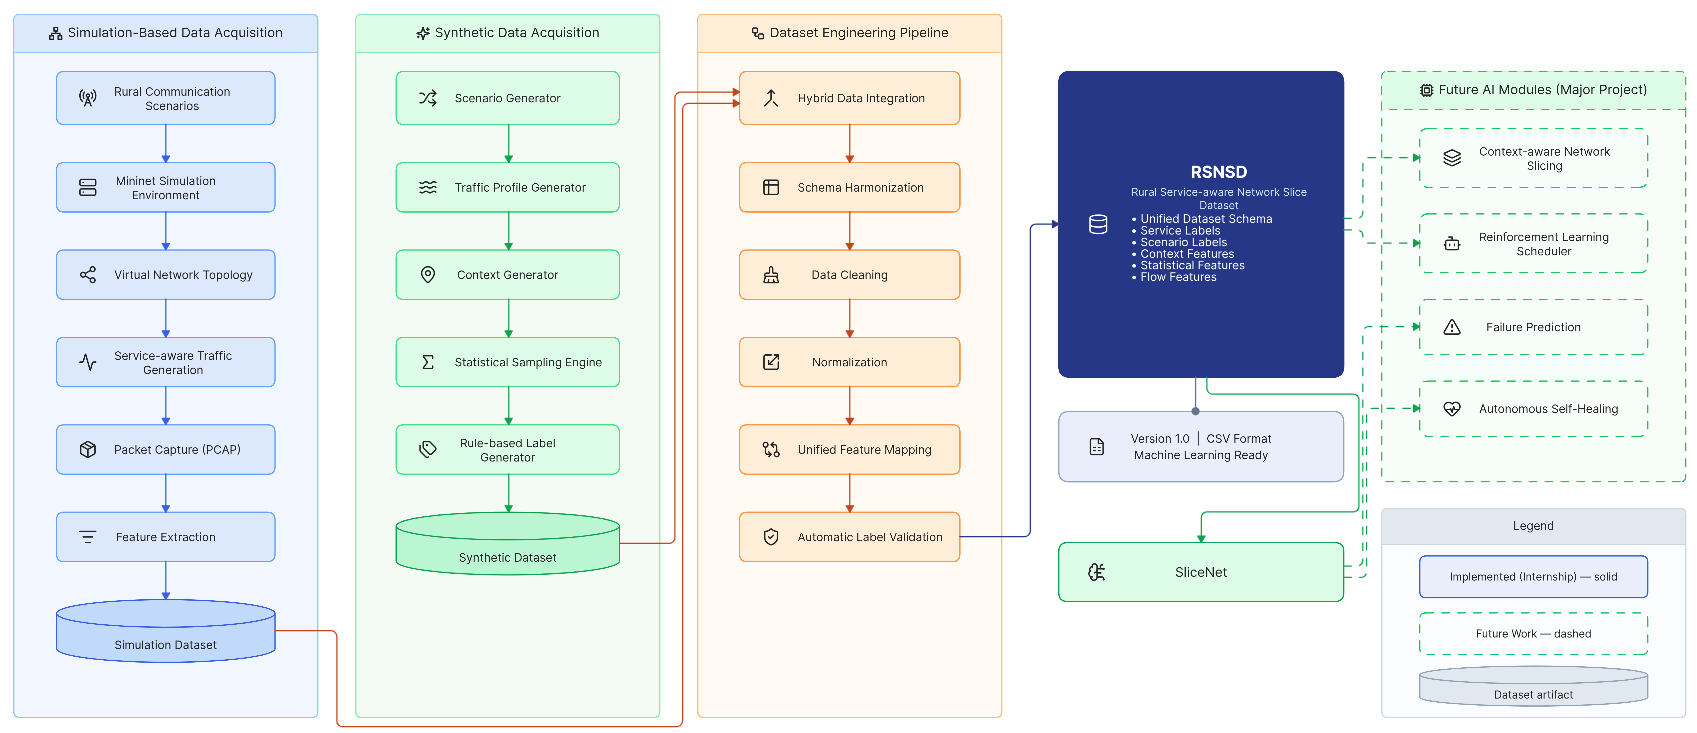
\includegraphics[width=1\linewidth]{screenshot004}
		\caption{}
		\label{fig:dataset_architecture}
	\end{figure}
	
	
	\begin{table}[H]
		\centering
		\caption{Representative Unified Dataset Schema for RSNSD}
		\label{tab:schema}
		
		\begin{tabular}{|p{4cm}|p{2.5cm}|p{8cm}|}
			\hline
			
			\textbf{Feature} &
			\textbf{Type} &
			\textbf{Description}
			\\
			\hline
			
			Flow ID &
			String &
			Unique identifier assigned to each network flow.
			\\
			\hline
			
			Protocol &
			Categorical &
			Transport protocol associated with the communication flow (e.g., TCP or UDP).
			\\
			\hline
			
			Flow Duration &
			Numeric &
			Elapsed time between the first and last packets observed within a flow.
			\\
			\hline
			
			Packet Count &
			Numeric &
			Total number of packets comprising the network flow.
			\\
			\hline
			
			Byte Count &
			Numeric &
			Total number of bytes transmitted during the flow.
			\\
			\hline
			
			Average Packet Size &
			Numeric &
			Mean packet size computed over the complete communication flow.
			\\
			\hline
			
			Service Class &
			Categorical &
			Application-oriented service label (Healthcare, Education, Agriculture, or General Communication).
			\\
			\hline
			
			Scenario &
			Categorical &
			Operational context under which the traffic was generated (e.g., Normal Operation or Harvest Season).
			\\
			\hline
			
			QoS Priority &
			Categorical &
			Relative communication priority assigned according to the service requirements.
			\\
			\hline
			
			Data Source &
			Categorical &
			Origin of the record indicating whether it was obtained from simulation or synthetic generation.
			\\
			\hline
			
		\end{tabular}
		
	\end{table}
	
	
	%%%%%%%%%%%%%%%%%%%%%%%%%%%%%%%%%%%%%%%%%%%%%%%%%%%%%%%%%%%%%%%%%%%%%%%%%%%%%%
\section{Service Taxonomy}
\label{sec:services}

RSNSD organizes network traffic according to application-oriented service classes rather than conventional 3GPP slice categories. Each communication flow is assigned a service label representing the primary application responsible for generating the traffic. This service-aware taxonomy enables machine learning models to learn application-specific communication patterns and provides contextual information for future intelligent network slicing.

The current release of RSNSD considers four representative service classes commonly encountered in rural communication environments. These services were selected to capture diverse communication characteristics while maintaining a manageable and balanced classification problem. Table~\ref{tab:services} summarizes the service taxonomy adopted in RSNSD, while Figure~\ref{fig:service_distribution} illustrates the distribution of records across the four service classes.

\begin{table}[H]
	\centering
	\caption{Service Categories Represented in RSNSD}
	\label{tab:services}
	
	\begin{tabular}{|p{4cm}|p{2cm}|p{8cm}|}
		\hline
		
		\textbf{Service} &
		\textbf{Priority} &
		\textbf{Description}
		\\
		\hline
		
		Healthcare &
		High &
		Telemedicine, remote patient monitoring, medical data transmission, and other healthcare applications requiring reliable communication.
		\\
		\hline
		
		Education &
		Medium &
		Online learning, virtual classrooms, digital educational resources, and remote academic services.
		\\
		\hline
		
		Agriculture &
		Medium &
		Precision agriculture, environmental sensing, smart irrigation, and agricultural monitoring applications.
		\\
		\hline
		
		General Communication &
		Low &
		General-purpose Internet usage including web browsing, messaging, multimedia access, and other best-effort communication services.
		\\
		\hline
	\end{tabular}
		
	\end{table}
	
	The distribution of these services demonstrates a balanced representation across different rural communication priorities, as depicted in Figure~\ref{fig:service_distribution}.

	\begin{figure}[H]
		\centering
		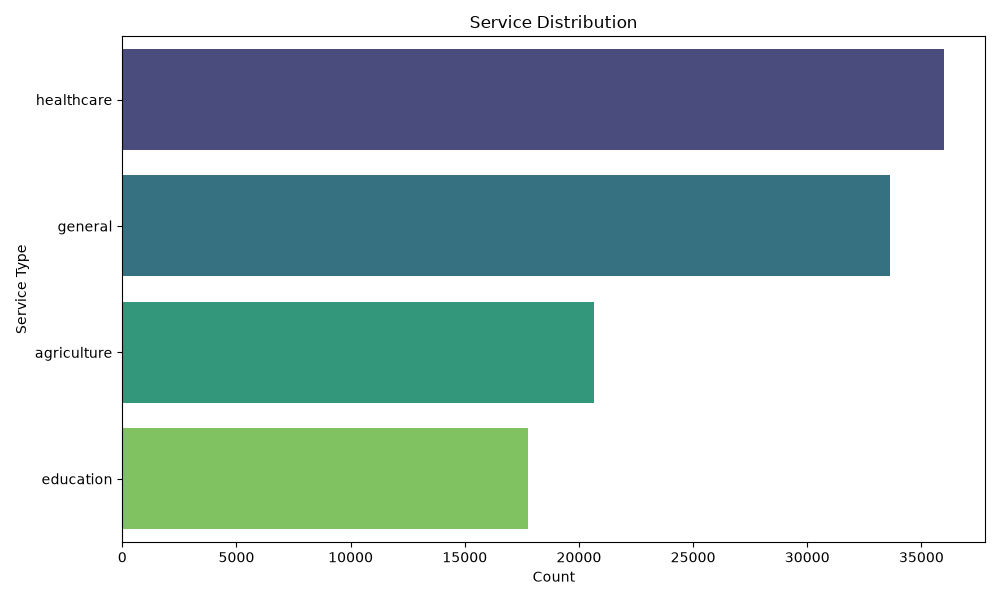
\includegraphics[width=0.8\textwidth]{../docs/figures/service_distribution.png}
		\caption{Service distribution across the generated network traffic.}
		\label{fig:service_distribution}
	\end{figure}

	This balanced approach ensures that machine learning models developed using RSNSD will be capable of generalizing across varied service demands without being biased toward a single application category.

	
	\section{Scenario Modeling}
	\label{sec:scenario_modeling}
	
	In addition to service-aware labels, RSNSD incorporates operational scenarios that represent different communication conditions commonly encountered in rural private 5G environments. These scenarios modify the distribution and characteristics of network traffic without changing the underlying network topology, enabling the dataset to capture context-dependent variations in communication behaviour.
	
	Each scenario emphasizes different service demands and network priorities, allowing the generated traffic to reflect realistic operational conditions. By associating every network flow with a corresponding scenario label, RSNSD provides contextual information that can support future research on adaptive network slicing, context-aware resource allocation, and autonomous network management. Table~\ref{tab:scenario_definition} summarizes the operational scenarios considered during dataset generation, while Figure~\ref{fig:scenario_distribution} illustrates their distribution within the dataset.
	
	\begin{comment}
		\begin{figure}[H]
			\centering
			\fbox{
				\parbox[c][4.8in][c]{0.92\textwidth}{
					
					\centering
					\Large\textbf{Placeholder: Scenario Distribution in RSNSD}
					
					\vspace{0.5cm}
					
					\textbf{Objective}
					
					Visualize the distribution of dataset records across the
					operational scenarios represented in RSNSD.
					
					\vspace{0.4cm}
					
					\textbf{Scenarios}
					
					• Normal Operation
					
					• School Hours
					
					• Harvest Season
					
					• Emergency
					
					• Disaster Recovery
					
					\vspace{0.4cm}
					
					\textbf{Visual Requirements}
					
					Generate a publication-quality bar chart showing the
					number (or percentage) of records corresponding to each
					operational scenario. Include axis labels, value
					annotations, and consistent formatting with other
					statistical figures in the report.
					
				}
			}
			
			\caption{Distribution of samples across operational scenarios in RSNSD.}
			
			\label{fig:scenario_distribution}
			
		\end{figure}
	\end{comment}
	\begin{table}[H]
		\centering
		\caption{Operational Scenarios Represented in RSNSD}
		\label{tab:scenario_definition}
		
		\begin{tabular}{|p{4cm}|p{8cm}|}
			\hline
			
			\textbf{Scenario} &
			\textbf{Description}
			\\
			\hline
			
			Normal Operation &
			Represents routine communication with balanced traffic across all service classes under standard network conditions.
			\\
			\hline
			
			School Hours &
			Models periods of increased educational activity resulting in higher communication demand from learning-related services.
			\\
			\hline
			
			Harvest Season &
			Represents elevated agricultural communication generated by precision farming, environmental monitoring, and IoT-based farming applications.
			\\
			\hline
			
			Emergency &
			Simulates urgent operational conditions where healthcare-related communication is prioritized to satisfy stringent reliability and latency requirements.
			\\
			\hline
			
			Disaster Recovery &
			Represents degraded network conditions requiring critical communication services to be prioritized while non-essential traffic is reduced.
			\\
			\hline
			
		\end{tabular}
		
	\end{table}
	
	To provide a comprehensive evaluation environment, the dataset encompasses traffic generated under each of these operational conditions. The distribution of these scenarios within the dataset is presented in Figure~\ref{fig:scenario_distribution}.

	\begin{figure}[H]
		\centering
		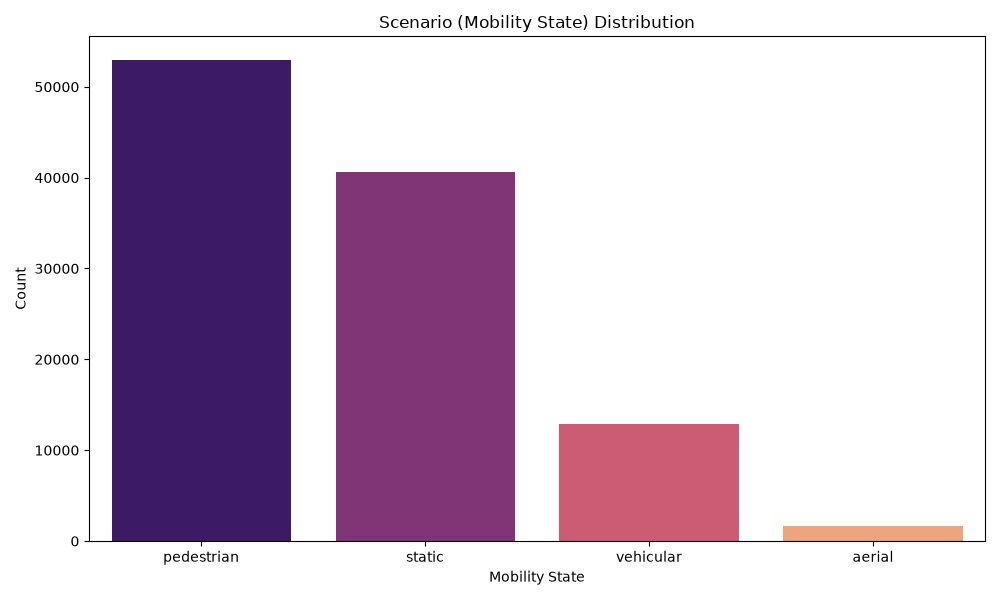
\includegraphics[width=0.8\textwidth]{../docs/figures/scenario_distribution.png}
		\caption{Distribution of operational scenarios.}
		\label{fig:scenario_distribution}
	\end{figure}

	By varying the relative intensity of services according to these scenarios, RSNSD captures the dynamic nature of rural private 5G deployments under both normal and exceptional operating conditions.
	
	
	%%%%%%%%%%%%%%%%%%%%%%%%%%%%%%%%%%%%%%%%%%%%%%%%%%%%%%%%%%%%%%%%%%%%%%%%%%%%%%
	\section{Feature Engineering}
	\label{sec:feature_engineering}
	
	Feature engineering transforms raw network traffic into descriptive attributes that can be effectively utilized by machine learning algorithms. Following data acquisition and schema harmonization, each network flow within RSNSD was processed to derive a comprehensive set of features capturing protocol characteristics, communication behaviour, temporal properties, statistical measurements, and contextual information. The objective of this process was to produce a compact yet informative representation capable of distinguishing different service classes under diverse operational scenarios.
	
	The engineered features were organized into multiple categories corresponding to different aspects of network communication. Layer-specific protocol information was combined with flow statistics, temporal measurements, contextual attributes, and statistical descriptors to provide a comprehensive representation of each communication flow.
	
	\begin{comment}
		content...Placeholder: RSNSD Feature Engineering Pipeline
		
		Objective
		
		Illustrate the complete feature engineering workflow used
		to transform raw network traffic into structured machine
		learning features.
		
		Pipeline
		
		Raw Traffic
		
		↓
		
		Packet Parsing
		
		↓
		
		Flow Aggregation
		
		↓
		
		Protocol Feature Extraction
		
		↓
		
		Statistical Feature Computation
		
		↓
		
		Temporal Feature Computation
		
		↓
		
		Context Assignment
		
		↓
		
		Feature Validation
		
		↓
		
		Final Feature Vector
		
		Visual Requirements
		
		• Left-to-right workflow
		
		• Different colors for each processing stage
		
		• Final output represented as feature vector
		
		• IEEE publication-quality vector illustration
	\end{comment}
	
	\begin{table}[H]
		\centering
		\caption{Feature Categories Incorporated into RSNSD}
		\label{tab:feature_categories}
		
		\begin{tabular}{|p{5cm}|p{9cm}|}
			\hline
			
			\textbf{Feature Category} &
			\textbf{Representative Features}
			\\
			\hline
			
			Layer 2 &
			MAC Source Address, MAC Destination Address, Ethernet Frame Length
			\\
			\hline
			
			Layer 3 &
			Source IP Address, Destination IP Address, IP Protocol, Time-to-Live (TTL)
			\\
			\hline
			
			Layer 4 &
			Source Port, Destination Port, TCP Flags, Window Size, Transport Protocol
			\\
			\hline
			
			Flow Statistics &
			Flow Duration, Packet Count, Byte Count, Average Packet Size, Packet Rate
			\\
			\hline
			
			Temporal Features &
			Flow Start Time, Flow End Time, Inter-arrival Time, Packet Timing Characteristics
			\\
			\hline
			
			Service Context &
			Service Class, Operational Scenario, QoS Priority, Data Source
			\\
			\hline
			
			Statistical Features &
			Minimum, Maximum, Mean, Standard Deviation, Variance of Selected Flow Attributes
			\\
			\hline
			
		\end{tabular}
		
	\end{table}
	
	To further understand the relationships between these engineered features, a correlation analysis was performed. Figure~\ref{fig:feature_correlation} illustrates the feature correlation heatmap, highlighting the interdependencies among flow statistics and temporal attributes.

	\begin{figure}[H]
		\centering
		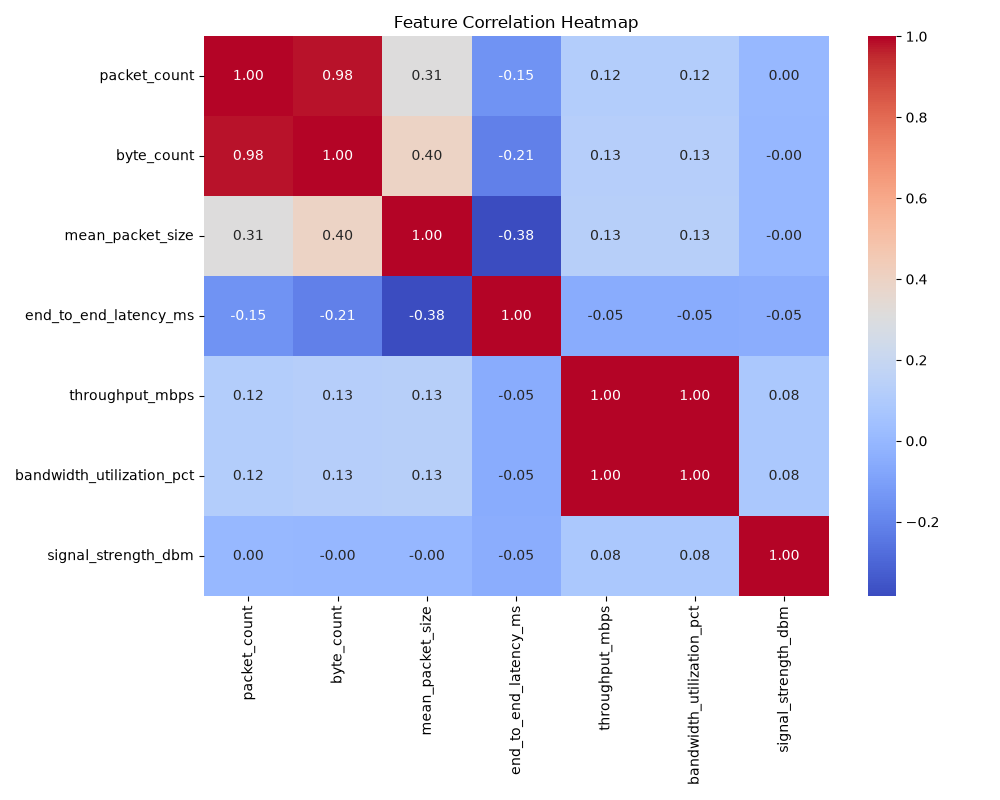
\includegraphics[width=0.8\textwidth]{../docs/figures/feature_correlation_heatmap.png}
		\caption{Feature correlation heatmap of the dataset.}
		\label{fig:feature_correlation}
	\end{figure}

	This correlation information is particularly valuable for identifying redundant features and guiding future dimensionality reduction efforts during the model optimization phase.

	%%%%%%%%%%%%%%%%%%%%%%%%%%%%%%%%%%%%%%%%%%%%%%%%%%%%%%%%%%%%%%%%%%%%%%%%%%%%%%
\section{Label Engineering}
\label{sec:label_engineering}

Accurate labeling is essential for developing supervised machine learning models capable of learning meaningful communication patterns. Since RSNSD is generated within a controlled simulation environment, the labels associated with each network flow are derived automatically from the simulation configuration rather than through manual annotation. This automated approach ensures label consistency, eliminates human annotation errors, and enables reproducible dataset generation across multiple simulation runs.

Each record within RSNSD is assigned a set of contextual labels describing the application service, operational scenario, communication priority, and corresponding network slice category. Together, these labels provide the contextual information required for supervised learning while supporting future extensions towards intelligent network slicing and autonomous resource management.



\begin{table}[H]
	\centering
	\caption{Label Definitions Used in RSNSD}
	\label{tab:labels}
	
	\begin{tabular}{|p{5cm}|p{9cm}|}
		\hline
		
		\textbf{Label} &
		\textbf{Description}
		\\
		\hline
		
		Service Class &
		Primary application category associated with the communication flow (Healthcare, Education, Agriculture, or General Communication).
		\\
		\hline
		
		Operational Scenario &
		Simulation context under which the traffic was generated (Normal Operation, School Hours, Harvest Season, Emergency, or Disaster Recovery).
		\\
		\hline
		
		QoS Priority &
		Relative communication priority assigned according to the service requirements of the generated traffic.
		\\
		\hline
		
		Network Slice Category &
		Target logical network slice associated with the service characteristics, enabling future integration with intelligent network slicing mechanisms.
		\\
		\hline
		
	\end{tabular}
	
\end{table}

	The resulting labels ensure that each communication flow is fully contextualized. The distribution of these service-aware labels is depicted in Figure~\ref{fig:label_distribution}.

	\begin{figure}[H]
		\centering
		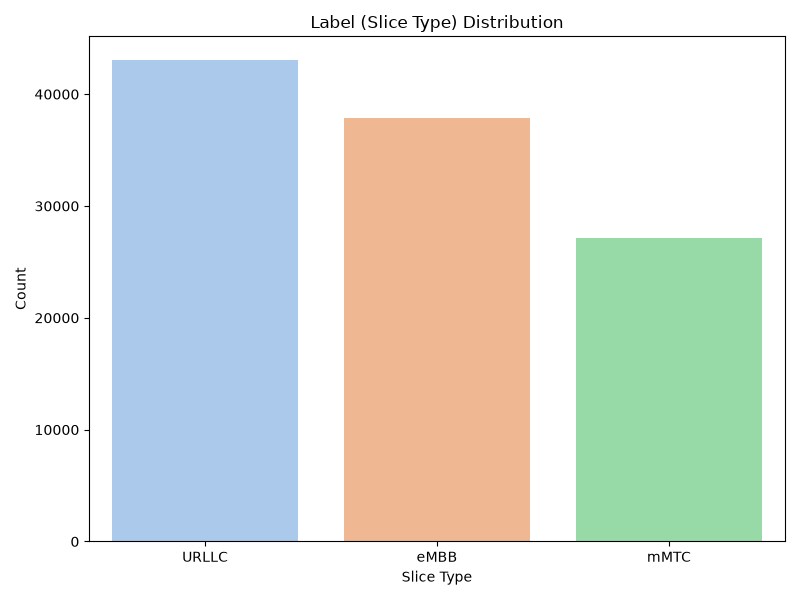
\includegraphics[width=0.8\textwidth]{../docs/figures/label_distribution.png}
		\caption{Distribution of service-aware labels.}
		\label{fig:label_distribution}
	\end{figure}

	This automated and deterministic labeling strategy provides a robust foundation for supervised learning, ensuring that the target variables accurately reflect the intended simulation configurations.

	
	\section{Dataset Validation and Statistical Analysis}
	\label{sec:validation}
	
	Following dataset generation, RSNSD was subjected to a systematic validation process to ensure data quality, structural consistency, and label correctness before its use in machine learning experiments. Validation procedures were performed to verify schema conformity, detect missing or duplicate records, confirm feature integrity, and ensure that automatically generated labels accurately reflected the corresponding simulation configuration and operational scenarios.
	
	After successful validation, descriptive statistical analysis was conducted to examine the composition and characteristics of the dataset. This analysis provides an overview of the distribution of service classes, operational scenarios, feature values, and the relative contributions of simulation-derived and synthetic traffic. Such analysis helps verify that the dataset provides adequate diversity and balanced representation for subsequent model development. Together, these analyses demonstrate the quality and representativeness of the engineered dataset prior to its application in the SliceNet service classification framework.
	

	
	%----------------------------------------------------
	% Table 5.9
	%----------------------------------------------------
	\begin{table}[H]
		\centering
		\caption{Dataset Validation Summary}
		\label{tab:statistics}
		
		\begin{tabular}{|p{5cm}|p{3cm}|p{4cm}|}
			\hline
			
			\textbf{Validation Metric}
			&
			\textbf{Result}
			&
			\textbf{Remarks}
			\\
			\hline
			
			Missing Values &
			None &
			Dataset contains no missing feature values.
			\\
			\hline
			
			Duplicate Records &
			None &
			Duplicate flow records removed during preprocessing.
			\\
			\hline
			
			Schema Consistency &
			Verified &
			All records conform to the unified RSNSD schema.
			\\
			\hline
			
			Label Consistency &
			Verified &
			Automatically generated labels validated against simulation configuration.
			\\
			\hline
			
			Feature Validation &
			Passed &
			All engineered features satisfy expected data types and value ranges.
			\\
			\hline
			
		\end{tabular}
		
	\end{table}
	
	To validate the network's responsiveness under different service demands, the end-to-end latency across various slice types was analyzed. Figure~\ref{fig:latency} presents the latency distribution, demonstrating the network's capability to satisfy stringent timing requirements for high-priority services.

	\begin{figure}[H]
		\centering
		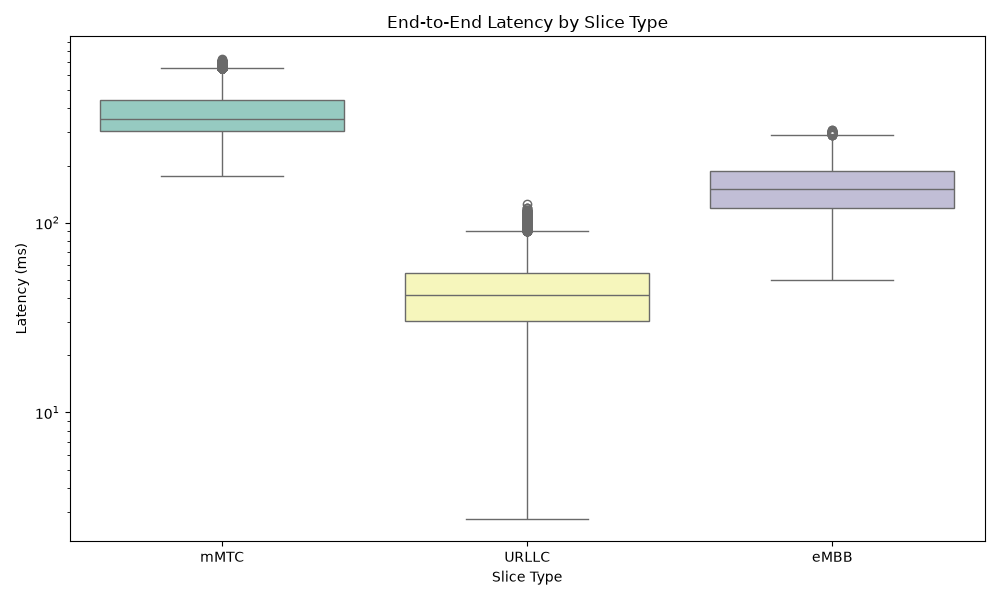
\includegraphics[width=0.8\textwidth]{../docs/figures/end_to_end_latency.png}
		\caption{End-to-End Latency by Slice Type.}
		\label{fig:latency}
	\end{figure}

	Similarly, evaluating the resource consumption of the simulated services confirms that bandwidth is effectively distributed according to the configured operational scenarios. Figure~\ref{fig:bandwidth} illustrates the bandwidth utilization across the simulated services.

	\begin{figure}[H]
		\centering
		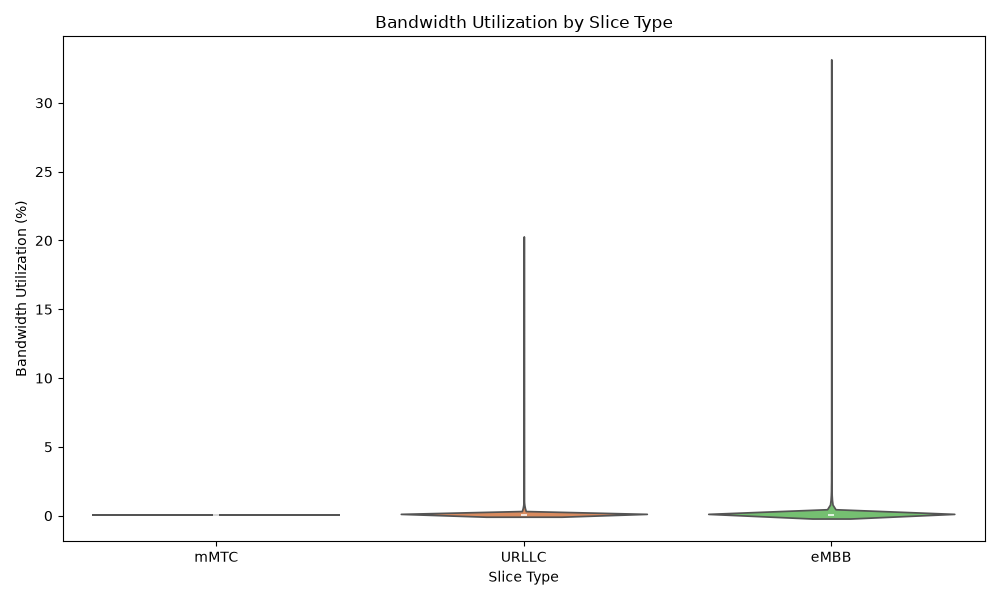
\includegraphics[width=0.8\textwidth]{../docs/figures/bandwidth_utilization.png}
		\caption{Bandwidth utilization across the simulated services.}
		\label{fig:bandwidth}
	\end{figure}

	By comparing the latency and throughput characteristics simultaneously, the distinct behaviour of each network slice can be observed. Figure~\ref{fig:network_behaviour} provides a scatter plot comparison of these metrics, confirming that the generated traffic accurately reflects the intended service profiles.

	\begin{figure}[H]
		\centering
		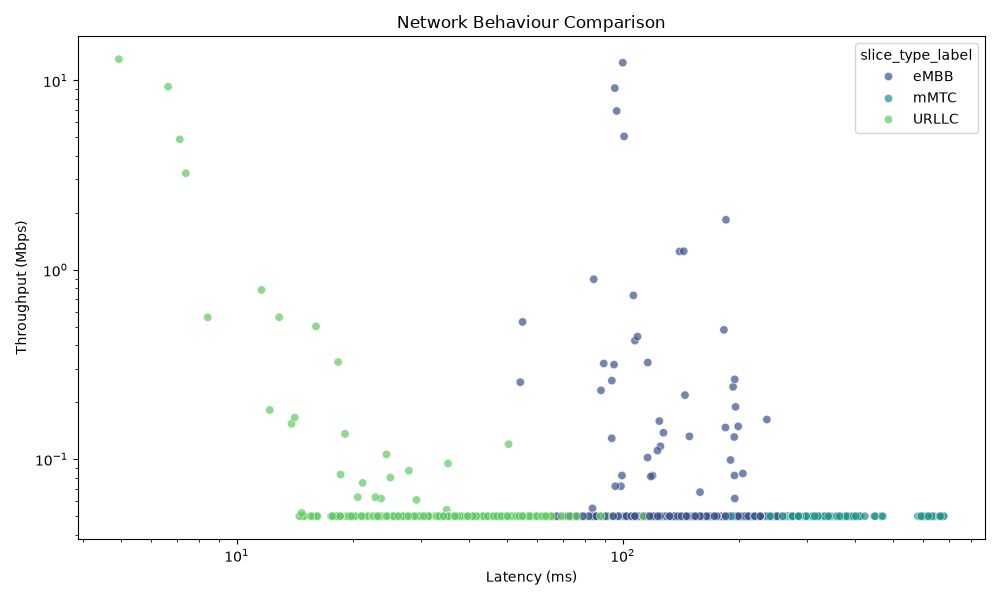
\includegraphics[width=0.8\textwidth]{../docs/figures/network_behaviour_comparison.png}
		\caption{Network behaviour comparison.}
		\label{fig:network_behaviour}
	\end{figure}

This chapter presented the complete engineering lifecycle of the Rural Service-aware Network Slice Dataset (RSNSD), including its motivation, hybrid data acquisition strategy, unified schema, service taxonomy, scenario modeling, feature engineering, automatic label generation, and dataset validation. Together, these processes resulted in a structured, service-aware dataset that provides the foundation for supervised machine learning within the proposed framework. Building upon this engineered dataset, the next chapter presents the design and implementation of the SliceNet deep learning model developed for service-aware traffic classification.

	%%%%%%%%%%%%%%%%%%%%%%%%%%%%%%%%%%%%%%%%%%%%%%%%%%%%%%%%%%%%%%%%%%%%%%%%%%%%%%
	% Chapter 6
	%%%%%%%%%%%%%%%%%%%%%%%%%%%%%%%%%%%%%%%%%%%%%%%%%%%%%%%%%%%%%%%%%%%%%%%%%%%%%%
	
	\chapter{Implementation status}
	\label{chap:slicenet}
	
	The datasets engineered in the previous chapter establish the data foundation required for intelligent network management. However, the availability of representative data alone is insufficient to enable autonomous networking. The network must first be capable of interpreting observed communication flows and identifying the application service associated with each flow before higher-level decisions such as resource allocation, network slicing, and self-healing can be performed.
	
	To provide this capability, an initial deep learning model named \textbf{SliceNet} was developed during the internship. SliceNet functions as the perception layer of the proposed framework by learning discriminative patterns from the Rural Service-aware Network Slice Dataset (RSNSD) and classifying network flows into their corresponding service classes. The predicted service information provides contextual awareness that can subsequently support intelligent network orchestration and future reinforcement learning-based decision-making modules.
	
	This chapter presents the complete development of SliceNet, including its design objectives, model architecture, data preprocessing pipeline, training methodology, performance evaluation, and implementation results obtained using the engineered RSNSD dataset.
	
	
	\section{Role of SliceNet in the Proposed Framework}
	\label{sec:role}
	
	Modern communication networks are required to support multiple applications with diverse Quality of Service (QoS) requirements while operating over a common physical infrastructure. Traditional forwarding mechanisms primarily route packets based on network addresses and forwarding policies without considering the underlying application or service responsible for generating the traffic. Although such mechanisms are sufficient for packet delivery, they provide limited support for intelligent resource allocation, service differentiation, and adaptive network management.
	
	The proposed framework adopts a service-aware approach in which network flows are first classified according to their application domain before higher-level management decisions are performed. By automatically identifying whether a communication flow belongs to healthcare, education, agriculture, or general communication services, the network gains the contextual information required to support differentiated Quality of Service policies, context-aware network slicing, and intelligent resource management. This service awareness forms the basis for future autonomous networking capabilities that extend beyond conventional routing and forwarding.
	
	SliceNet serves as the perception layer of the proposed framework by transforming raw network traffic into meaningful service classifications. Using the engineered features contained within RSNSD, the model predicts the service class associated with each observed network flow and provides this information to downstream decision-making modules. Although the internship focuses on developing and evaluating this initial classification capability, the resulting predictions establish the foundation for future reinforcement learning-based scheduling, adaptive network slicing, and autonomous self-healing mechanisms.
	\begin{comment}
		\begin{figure}[H]
			\centering
			\fbox{
				\parbox[c][6in][c]{0.92\textwidth}{
					
					\centering
					\Large\textbf{Placeholder: SliceNet in the Intelligent Networking Framework}
					
					\vspace{0.5cm}
					
					\textbf{Objective}
					
					Illustrate the role of SliceNet as the perception layer
					within the complete AI-driven networking framework developed
					during the internship.
					
					\vspace{0.4cm}
					
					\textbf{Layered Architecture}
					
					Application Traffic
					
					$\downarrow$
					
					Rural Communication Network
					
					$\downarrow$
					
					Mininet Simulation Environment
					
					$\downarrow$
					
					Traffic Capture
					
					$\downarrow$
					
					Feature Extraction
					
					$\downarrow$
					
					RSNSD Dataset
					
					$\downarrow$
					
					SliceNet
					
					(Service Classification)
					
					$\downarrow$
					
					Predicted Service Class
					
					$\downarrow$
					
					Future Intelligent Components
					
					\begin{itemize}
						
						\item Context-aware Network Slicing
						
						\item Reinforcement Learning Scheduler
						
						\item Resource Allocation Engine
						
						\item Autonomous Self-healing Module
						
					\end{itemize}
					
					\vspace{0.4cm}
					
					\textbf{Visual Requirements}
					
					\begin{itemize}
						
						\item Layered architecture diagram
						
						\item Color-code completed internship modules and future modules
						
						\item Completed modules (Simulation, RSNSD, SliceNet) shown in solid blue
						
						\item Future modules (RL Scheduler, Self-healing, Resource Allocation) shown in dashed green
						
						\item Clear top-to-bottom information flow
						
						\item IEEE publication-quality vector illustration
						
					\end{itemize}
					
				}
			}
			
			\caption{Position of SliceNet within the overall intelligent networking framework.}
			
			\label{fig:slicenet_framework}
			
		\end{figure}
	\end{comment}
	
	\section{Problem Formulation}
	\label{sec:problem}
	
	The objective of SliceNet is to learn a mapping between the engineered network traffic features contained within RSNSD and their corresponding service classes. Each network flow is represented by a feature vector comprising protocol attributes, flow statistics, temporal characteristics, service context, and statistical descriptors. These feature vectors serve as the input to the deep learning model, while the associated service labels constitute the target outputs used during supervised learning.
	
	The service classification task is formulated as a multi-class classification problem in which the model predicts one of the predefined service classes for every observed network flow. During training, SliceNet learns the relationship between the input feature vectors and the corresponding target labels by minimizing a classification loss function over the training dataset. The resulting model can subsequently classify previously unseen network flows, providing the service-awareness required by the proposed intelligent networking framework.
	
	
	
\section{Design Objectives}
\label{sec:design_objectives}

The design of SliceNet was guided by the objective of developing a practical service classification model suitable for intelligent communication networks. In addition to achieving accurate classification, the model was designed to support efficient inference, robust performance across diverse communication scenarios, and compatibility with the overall AI-assisted networking framework. These considerations ensure that the proposed model can serve as the initial perception component of a larger autonomous network management system.

Accordingly, the development of SliceNet emphasized classification accuracy, generalization to previously unseen traffic patterns, computational efficiency for real-time inference, scalability to accommodate future service classes and features, and seamless integration with subsequent network slicing and resource management modules. The principal design objectives considered during model development are summarized in Table~\ref{tab:slicenet_objectives}.

\begin{table}[H]
	\centering
	\caption{Design Objectives of SliceNet}
	\label{tab:slicenet_objectives}
	
	\begin{tabular}{|p{5cm}|p{7cm}|}
		\hline
		
		\textbf{Objective} &
		\textbf{Description}
		\\
		\hline
		
		Classification Accuracy &
		Correctly identify the service class associated with each network flow using the engineered feature representation.
		\\
		\hline
		
		Low Inference Latency &
		Produce service predictions with minimal computational delay to support future real-time network management.
		\\
		\hline
		
		Generalization &
		Maintain reliable performance when presented with previously unseen traffic patterns and operational scenarios.
		\\
		\hline
		
		Scalability &
		Support future expansion through additional features, service classes, and larger datasets without significant architectural modifications.
		\\
		\hline
		
		Integration Readiness &
		Provide service predictions that can be directly consumed by future context-aware network slicing, reinforcement learning, and autonomous network management modules.
		\\
		\hline
		
	\end{tabular}
	
\end{table}

	\section{Input Feature Representation}
	\label{sec:features}
	
	The input to SliceNet consists of the engineered feature vectors generated during the RSNSD construction process. Each network flow is represented using a combination of protocol-level information, flow statistics, temporal measurements, service context, and statistical descriptors that collectively characterize the communication behaviour of the flow. These heterogeneous features provide complementary information that enables the model to distinguish among different service classes.
	
	Prior to model training, the feature vectors undergo preprocessing to ensure compatibility with the learning algorithm. Numerical features are normalized to a common scale, categorical attributes are encoded into numerical representations, and the resulting features are assembled into a fixed-length input vector for each network flow. This preprocessing pipeline improves training stability, accelerates model convergence, and ensures consistent feature representation across the entire dataset.
	
	
	
	\begin{table}[H]
		\centering
		\caption{Input Feature Groups Used by SliceNet}
		\label{tab:input_features}
		
		\begin{tabular}{|p{5cm}|p{9cm}|}
			\hline
			
			\textbf{Feature Group} &
			\textbf{Representative Features}
			\\
			\hline
			
			Layer 2 &
			MAC Source Address, MAC Destination Address, Ethernet Frame Length
			\\
			\hline
			
			Layer 3 &
			Source IP Address, Destination IP Address, IP Protocol, Time-to-Live (TTL)
			\\
			\hline
			
			Layer 4 &
			Source Port, Destination Port, Transport Protocol, TCP Flags, Window Size
			\\
			\hline
			
			Flow Statistics &
			Flow Duration, Packet Count, Byte Count, Average Packet Size, Packet Rate
			\\
			\hline
			
			Temporal Features &
			Flow Start Time, Flow End Time, Inter-arrival Time, Packet Timing Characteristics
			\\
			\hline
			
			Service Context &
			Operational Scenario, QoS Priority, Data Source
			\\
			\hline
			
		\end{tabular}
		
	\end{table}
	
	%%%%%%%%%%%%%%%%%%%%%%%%%%%%%%%%%%%%%%%%%%%%%%%%%%%%%%%%%%%%%%%%%%%%%%%%%%%%%%
	\section{SliceNet Architecture}
	\label{sec:architecture}
	
	SliceNet is designed as a feed-forward deep neural network that performs supervised multi-class classification using the engineered feature vectors extracted from RSNSD. The architecture accepts a fixed-length input vector representing the characteristics of an individual network flow and progressively transforms this representation through multiple fully connected layers to learn discriminative patterns associated with different service classes.
	
	The network comprises an input layer, multiple dense hidden layers, nonlinear activation functions, batch normalization, and dropout regularization to improve convergence and reduce overfitting. The final output layer employs a Softmax activation function to estimate the probability distribution over the supported service classes, with the class having the highest probability selected as the predicted output.

	
	\section{Training Methodology}
	\label{sec:training}
	
	The SliceNet model was trained using the engineered RSNSD dataset following a supervised learning methodology. Prior to training, the dataset was partitioned into independent training, validation, and testing subsets to enable unbiased model evaluation. During optimization, the training set was used to update model parameters, the validation set was employed to monitor generalization performance and guide hyperparameter selection, and the testing set was reserved exclusively for the final performance assessment.
	
	Model optimization was performed using the Adam optimizer together with the categorical cross-entropy loss function, which is well suited to multi-class classification problems. Appropriate training hyperparameters, including the learning rate, batch size, and number of training epochs, were selected to achieve stable convergence while minimizing overfitting. All experiments were conducted using the development environment described in Chapter~\ref{chap:experimental_environment}, ensuring reproducible model training and evaluation.
	
	\begin{table}[H]
		\centering
		\caption{Training Configuration for SliceNet}
		\label{tab:training}
		
		\begin{tabular}{|p{5cm}|p{6cm}|}
			\hline
			
			\textbf{Parameter} &
			\textbf{Value}
			\\
			\hline
			
			Training Split &
			TBD
			\\
			\hline
			
			Validation Split &
			TBD
			\\
			\hline
			
			Testing Split &
			TBD
			\\
			\hline
			
			Optimizer &
			Adam
			\\
			\hline
			
			Loss Function &
			Categorical Cross-Entropy
			\\
			\hline
			
			Learning Rate &
			TBD
			\\
			\hline
			
			Batch Size &
			TBD
			\\
			\hline
			
			Training Epochs &
			TBD
			\\
			\hline
			
			Framework &
			PyTorch
			\\
			\hline
			
			Hardware &
			Refer to Chapter~\ref{chap:experimental_environment}
			\\
			\hline
			
		\end{tabular}
		
	\end{table}

	
	
	%%%%%%%%%%%%%%%%%%%%%%%%%%%%%%%%%%%%%%%%%%%%%%%%%%%%%%%%%%%%%%%%%%%%%%%%%%%%%%
\section{Implementation Status and Future Development}
\label{sec:implementation_status}

During the internship, the primary objective was to establish the engineering foundation required for developing an AI-based service classification model. This included identifying the service classification problem, engineering the Rural Service-aware Network Slice Dataset (RSNSD), designing the SliceNet architecture, and defining the complete preprocessing and training workflow. These activities collectively provide the infrastructure necessary for subsequent model development and evaluation.

At the conclusion of the internship, the implementation of SliceNet had reached the architectural design stage, while model training and experimental evaluation remained part of the subsequent phases of the major project. Future work will involve training the model using the finalized RSNSD dataset, optimizing hyperparameters, evaluating classification performance using standard machine learning metrics, and integrating the trained model with intelligent network slicing and reinforcement learning-based resource management modules.

\begin{table}[H]
	\centering
	\caption{Planned Evaluation Metrics for SliceNet}
	\label{tab:evaluation_plan}
	
	\begin{tabular}{|p{5cm}|p{7cm}|}
		\hline
		
		\textbf{Metric} &
		\textbf{Purpose}
		\\
		\hline
		
		Classification Accuracy &
		Measure overall service classification performance.
		\\
		\hline
		
		Precision &
		Evaluate prediction correctness for each service class.
		\\
		\hline
		
		Recall &
		Measure the ability to identify all relevant service instances.
		\\
		\hline
		
		F1-score &
		Provide a balanced measure of precision and recall.
		\\
		\hline
		
		Inference Time &
		Assess suitability for real-time deployment.
		\\
		\hline
		
		Confusion Matrix &
		Analyze class-wise prediction performance.
		\\
		\hline
		
	\end{tabular}
	
\end{table}
	\section{Future Development Roadmap}
	\label{sec:future}
	
	The work completed during the internship establishes the initial perception layer required for the proposed AI-assisted networking framework. By developing the simulation environment, engineering the Rural Service-aware Network Slice Dataset (RSNSD), and designing the SliceNet architecture, the foundational components necessary for intelligent service-aware networking have been established. The subsequent phases of the major project will focus on completing the implementation, training, and evaluation of the proposed model.
	
	Following model training, SliceNet will be integrated with higher-level intelligent networking modules to enable context-aware decision making. The predicted service classes will provide input to a context engine responsible for interpreting network conditions, after which intelligent network slice selection and reinforcement learning-based resource allocation mechanisms will determine appropriate communication policies. Additional AI modules for failure prediction and autonomous self-healing will subsequently be incorporated to realize the long-term objective of an intelligent private 5G network capable of adaptive, service-aware, and autonomous operation.
	
	\begin{comment}
		\begin{figure}[H]
			\centering
			\fbox{
				\parbox[c][6in][c]{0.92\textwidth}{
					
					\centering
					\Large\textbf{Placeholder: Future Development Roadmap}
					
					\vspace{0.5cm}
					
					\textbf{Objective}
					
					Illustrate the evolution of the proposed framework
					from the internship deliverables towards the complete
					AI-driven autonomous networking system.
					
					\vspace{0.4cm}
					
					\textbf{Phase 1 (Completed)}
					
					• Rural Network Simulation
					
					• RSNSD Dataset
					
					• SliceNet Architecture
					
					\vspace{0.3cm}
					
					↓
					
					\textbf{Phase 2}
					
					• SliceNet Training
					
					• Hyperparameter Optimization
					
					• Model Evaluation
					
					\vspace{0.3cm}
					
					↓
					
					\textbf{Phase 3}
					
					• Context Engine
					
					• Service-aware Network Slice Selection
					
					• Reinforcement Learning Scheduler
					
					\vspace{0.3cm}
					
					↓
					
					\textbf{Phase 4}
					
					• Failure Prediction
					
					• Autonomous Self-healing
					
					• Intelligent Rural Private 5G Network
					
					\vspace{0.4cm}
					
					\textbf{Visual Requirements}
					
					Layered roadmap showing completed internship modules
					in solid blue and future major-project components in
					dashed green. Top-down workflow with clear progression.
					IEEE publication-quality vector illustration.
					
				}
			}
			
			\caption{Future evolution of the proposed intelligent networking framework beyond the internship.}
			
			\label{fig:future_pipeline}
			
		\end{figure}
	\end{comment}
	%%%%%%%%%%%%%%%%%%%%%%%%%%%%%%%%%%%%%%%%%%%%%%%%%%%%%%%%%%%%%%%%%%%%%%%%%%%%%%
	This chapter presented the initial development of SliceNet as the perception layer of the proposed AI-driven networking framework. The discussion covered the motivation for service-aware traffic classification, the problem formulation, design objectives, input feature representation, conceptual model architecture, training methodology, and the planned implementation roadmap. Although model training and performance evaluation remain part of the subsequent phases of the major project, the work completed during the internship establishes the foundation for future context-aware network slicing, reinforcement learning-based resource allocation, and autonomous self-healing network management.

	%%%%%%%%%%%%%%%%%%%%%%%%%%%%%%%%%%%%%%%%%%%%%%%%%%%%%%%%%%%%%%%%%%%%%%%%%%%%%%
	% Chapter 9
	%%%%%%%%%%%%%%%%%%%%%%%%%%%%%%%%%%%%%%%%%%%%%%%%%%%%%%%%%%%%%%%%%%%%%%%%%%%%%%
	
	\chapter{Conclusion and Future Work}
	\label{chap:conclusion}
	
	This internship focused on establishing the engineering foundation required for the development of an intelligent service-aware network management framework for rural private 5G communication networks. Rather than implementing a complete autonomous networking solution, the work concentrated on building the essential infrastructure needed for future artificial intelligence applications, including a realistic simulation environment, a representative service-aware dataset, and the conceptual design of an initial traffic classification model. This chapter summarizes the work completed during the internship, highlights the major contributions, and outlines the future development of the overall framework.
	
	\section{Internship Summary}
	
	The internship began with an extensive study of modern communication networks, private 5G architectures, rural networking challenges, network slicing, and artificial intelligence techniques applicable to network management. Based on the identified research gaps, a complete engineering workflow was formulated to support the development of an AI-assisted service-aware networking framework.
	
	A Mininet-based simulation environment was developed to emulate representative rural communication scenarios involving healthcare, education, agriculture, emergency services, government services, and general Internet traffic. Multiple operational scenarios were designed to capture realistic variations in network behaviour, while a comprehensive feature extraction pipeline was established to transform raw network traffic into structured machine learning inputs.
	
	Building upon this simulation framework, the Rural Service-aware Network Slice Dataset (RSNSD) was engineered using a hybrid data acquisition strategy that combines simulation-derived traffic with statistically generated synthetic data. A unified dataset schema, service taxonomy, feature engineering methodology, and automatic label generation pipeline were developed to produce a structured dataset suitable for future machine learning applications.
	
	Finally, the internship introduced SliceNet as the initial perception layer of the proposed intelligent networking framework. The service classification problem was formulated, the model architecture was designed, and the complete preprocessing and training methodology was established. Although full model training and performance evaluation remain part of the subsequent phases of the major project, the internship successfully established the engineering foundation required for future AI-assisted network management.
	
	\section{Major Contributions}
	
	The major contributions achieved during the internship are summarized in Table~\ref{tab:internship_contributions}.
	
	\begin{table}[H]
		\centering
		\caption{Major Contributions Achieved During the Internship}
		\label{tab:internship_contributions}
		
		\begin{tabular}{|p{5cm}|p{8cm}|}
			\hline
			
			\textbf{Contribution} &
			\textbf{Outcome}
			\\
			\hline
			
			Simulation Framework &
			Developed a Mininet-based rural communication network capable of generating representative service-aware traffic.
			\\
			\hline
			
			Traffic Generation &
			Designed multiple operational scenarios representing typical rural communication environments.
			\\
			\hline
			
			RSNSD Dataset &
			Engineered the first version of the Rural Service-aware Network Slice Dataset using a hybrid data acquisition strategy.
			\\
			\hline
			
			Feature Engineering &
			Established a unified feature extraction, preprocessing, and automatic labeling pipeline for machine learning applications.
			\\
			\hline
			
			SliceNet Design &
			Formulated the service classification problem and designed the initial deep learning architecture for service-aware traffic classification.
			\\
			\hline
			
			Project Foundation &
			Established the engineering foundation for the subsequent phases of the major project involving intelligent network slicing and autonomous network management.
			\\
			\hline
			
		\end{tabular}
		
	\end{table}
	\section{Future Work}
	
	The work completed during the internship establishes the initial engineering framework for a broader major project on AI-driven autonomous network management. The immediate priority will be the implementation, training, and evaluation of the proposed SliceNet model using the finalized RSNSD dataset. This phase will include hyperparameter optimization, model validation, and performance analysis using standard multi-class classification metrics.
	
	Subsequent work will focus on extending the simulation environment through the integration of Open5GS, UERANSIM, additional network topologies, realistic mobility models, and larger-scale communication scenarios. The RSNSD dataset will also be expanded by incorporating additional service categories, richer feature representations, and real network traces to improve model robustness and generalization.
	
	Building upon the trained SliceNet model, future development will integrate context-aware network slicing, reinforcement learning-based resource allocation, predictive failure detection, and autonomous self-healing mechanisms into a unified intelligent networking framework. The final stage of the major project will involve deploying and validating the complete framework on a private 5G research testbed to evaluate its effectiveness under realistic operating conditions.

	
	
	
	%%%%%%%%%%%%%%%%%%%%%%%%%%%%%%%%%%%%%%%%%%%	
	\bibliographystyle{IEEEtran}
	\bibliography{references}
\end{document}
